\documentclass[12pt]{article}
\usepackage[a4paper, margin=20mm, marginparwidth = 1.8cm]{geometry}
\usepackage{graphicx}
\usepackage{float}
\usepackage{fontspec}
\usepackage{booktabs}

\usepackage{url}
\usepackage{appendix}
\usepackage{subfigure}
\usepackage{bm}
\usepackage{amsfonts}
\usepackage{amsmath}
\usepackage{algorithm}
\usepackage{algpseudocode}

\usepackage{listings}
\usepackage{xcolor}

\usepackage[hidelinks]{hyperref}
\usepackage{ocgx2}

\newcounter{step}[subsubsection]
\renewcommand{\thestep}{\arabic{step}}
\newcommand{\step}{\refstepcounter{step}\textbf{Step \thestep:} }

\lstset{
    basicstyle=\ttfamily\footnotesize,
    keywordstyle=\color{blue},
    commentstyle=\color{gray},
    stringstyle=\color{red},
    numbers=left,
    numberstyle=\tiny,
    breaklines=true
}

\linespread{1.15}

\setmainfont{Times New Roman}
\pagenumbering{roman}

\begin{document}
\begin{titlepage}
	\centering
	\vspace*{3cm}
	\hrulefill\\
	\vspace{0.5cm}
	{\scshape\LARGE STAT5003 NOTE\par}
	\vspace{0.5cm}
	\hrulefill\\
	\vspace{1.5cm}

	{\normalsize\itshape Sheng\par}
	
	
	\vspace{14.5cm}
	{\normalsize 2025 \par}

\end{titlepage}

\input{contents}
\pagebreak

\section{Week 1}
\pagenumbering{arabic}
\subsection{Review of basic statistical concepts}

\noindent\textbf{Population}: The set of data (numeric or otherwise) corresponding to the entire collection of units about which information is sought.

\noindent\textbf{Sample}: A subset of the population data that are actually collected in the course of a study.

\subsubsection{Parameters vs Statistics}

\noindent\textbf{Parameter}: is a number that describes a population. Notation usually denoted with Greek letters, e.g. $\mu,\sigma$. A parameter is a fixed number (usually unknown).

\noindent\textbf{Statistic}: is a number that describes a sample. Sample statistics are usually denoted using Roman letters, e.g. $x,s$. A statistic is a variable whose value varies from sample to sample.

\subsubsection{Descriptive statistics – numeric and graphics}

\indent

Many methods are available for summarising data in both numeric and graphical form

Numeric measures:

\begin{itemize}
    \item Measure of location: Mean, Median, Mode for numeric data; Counts, proportions for categorical data.
    \item Measure of spread: Standard deviation, MAD (median absolute deviation), IQR (interquartile range)
    \item Others: Min, Max, Quartile, Five number summaries (used later in boxplot)
\end{itemize}

\subsubsection{Homogeneous vs non-homogenous data types}

\noindent\textbf{Homogeneous}

\begin{itemize}
    \item Vector: Sequence of data elements of the same basic data type
    \item Matrix: Collection of data elements in a 2-dimensional array with rows and columns
\end{itemize}

\noindent\textbf{Non-homogeneous}

\begin{itemize}
    \item List: More general structure containing other objects (including possibly other lists)
    \item Data frame: Used for storing data, each column can be a different basic type. All columns must have the same length.
\end{itemize}




\pagebreak

\section{Week 2}
\subsection{Statistical Learning}

\noindent\textbf{Statistical learning}: A field within statistics that focuses on \textbf{building models} to \textbf{make predictions or inferences}.

\noindent\textbf{Supervised Learning}: Given a dataset with features/predictors $(X_1,X_2,...,X_p)$ and a target outcome variable $(Y)$, the goal is to learn a model $f(X_1,...,X_p)$ to explain/predict the target.

\noindent\textbf{Unsupervised Learning}: Given a dataset with features $(X_1,X_2,...,X_p)$ the goal is to visualise, find patterns, subgroups/clusters within the data.

\subsubsection{Supervised Learning}

\noindent\textbf{Regression}: $Y = f(X)+\epsilon$.

$\epsilon$ is the irreducible error.

The main task is to use the sample to estimate $f(X)$.

\noindent\textbf{Parametric regression}: $f(X) = \beta_0+\beta_1 X_{i1}+...+\beta_p X_{ip}$

\noindent\textbf{Non-parametric regression}:

\begin{itemize}
    \item Does not make explicit assumption about the function form about $f(X)$.
    \item Assumes $f(X)$ is a smooth function that fits the data well.
\end{itemize}

\subsection{Simple Linear Regression}

\begin{align*}
    Y = f(X)+\epsilon = \beta_0+\beta_1 X+\epsilon
\end{align*}

\begin{itemize}
    \item $X$ is the predictor (feature or independent variable).
    \item $Y$ is the response (target or dependent variable).
    \item $\beta_0$ is the intercept of the regression line. Expected value of $Y$ when $X=0$.
    \item $\beta_1$ is the slope of the regression line. Mean increase in $Y$ for a unit increase in $X$.
    \item $\epsilon$ is the irreducible or random error. Classically assumed to be normally distributed with mean zero and finite variance
\end{itemize}

\subsubsection{Criterion to Measure the Notion}

\indent 

Easiest mathematical solution is the least squares criterion.

\begin{itemize}
    \item Let $\hat{y_i}$ be the estimated mean of $Y$ given $X=x_i$.
    \item Minimise the residual sum of squares $\text{RSS} = \sum_{i=1}^{n}(y_i - \hat{y_i})^2 = \sum_{i=1}^{n}e_i^2$.
    \item Recall we assume the noises are iid; if the variance of the residual term varies widely, we have the heteroskedastic issue.
\end{itemize}

\subsubsection{Least Squares Equations}

\noindent\textbf{Regression (slope) coefficient}:

\begin{align*}
    b_1 = \frac{\sum_{i=1}^{n}(x_i - \bar{x})(y_i - \bar{y})}{\sum_{i=1}^{n}(x_i-\bar{x})^2} = \frac{\text{Cov}(x,y)}{\text{Var}(x)}
\end{align*}

\noindent\textbf{Intercept}: $b_0 = \bar{y}-b_1 x$

\noindent\textbf{The estimated regression line}:

\begin{align*}
    \bar{y} = \widehat{f(x)} = b_0 + b_1 x
\end{align*}

Under conditions below, the least square estimator is the best linear unbiased estimator

\begin{itemize}
    \item Linearity, no multicollinearity, strict exogeneity
    \item Normal distributed errors (more generally, spherical errors)
\end{itemize}

\subsection{Basic uses of Simple Linear Regression}

\subsubsection{Standard error of sample mean}

\indent

Consider a single population estimation problem, wish to estimate some mean, $\mu$ of some random variable $Y$.

If $Y_1,...,Y_n$ are sampled then $\hat{\mu} = \bar{Y}=\sum_{i=1}^{n}Y_i/n$ is an estimator of $\mu$ with:

\begin{align*}
    \text{Var}(\hat{\mu})=(\text{SE}(\hat{\mu}))^2 = \frac{\sigma^2}{n}
\end{align*}

\subsubsection{Standard error of regression coefficient estimates}

\indent 

Same concept applies to the regression estimates:

\begin{align*}
    & \text{SE}(\widehat{\beta_0}) = \sigma\sqrt{\frac{1}{n}+\frac{\bar{x}^2}{\sum_{i=1}^{n}(x_i-\bar{x})^2}}\\
    & \text{SE}(\widehat{\beta_1})= \frac{\sigma}{\sqrt{\sum_{i=1}^{n}(x_i-\bar{x})^2}}
\end{align*}

where $\sigma ^2 = \text{Var}(\epsilon)$

As $n\xrightarrow[]{}\infty$, $\text{SE}(\widehat{\beta_0})\xrightarrow{}0$, $\text{SE}(\widehat{\beta_1})\xrightarrow{}0$.

Interestingly, if the $x_i$ are more spread out, the standard errors will be smaller (more leverage to estimate the parameters).

\subsubsection{Assessing the Model Fit–Goodness of fit statistic}

\indent 

Goodness of fit is measured by the coefficient of determination or $R^2$

\begin{align*}
    R^2 &= \frac{\text{SST} - \text{SSR}}{\text{SST}} = \frac{\text{SSE}}{\text{SST}}\\
     & = \frac{\sum_{i=1}^n(y_i - \bar{y})^2-\sum_{i=1}^{n}(y_i - \hat{y_i})^2}{\sum_{i=1}^n(y_i-\bar{y})^2}
\end{align*}

$R^2$ is a measure between 0 and 1 for the training dataset. It measures the proportion of variation in the response $Y$, explained by the linear regression on $X$.

\begin{itemize}
    \item $R^2 = 0$ indicates none of the variance in $Y$ can be explained linearly by $X$.
    \item $R^2 = 1$ indicates all of the variance in $Y$ can be explained linearly by $X$.
\end{itemize}

$R^2$ is \textbf{NOT suggested} (or at least not used as the only metric) for evaluating nonlinear models (introduced in subsequent weeks). Because Total Sum of Squares is NOT the summation of Residual Sum of Squares and Explained Sum of Squares for nonlinear models.

\subsection{Extending Simple Linear Regression}

\begin{align*}
    \text{Example}: Y = \beta_0+\beta_1X_1+\beta X_1 X_2 + \beta_3 X_2 +...
\end{align*}

Sometimes it is the case that an interaction term has a very small $p$-value, but the associated main effects do not.

\textbf{The hierarchy principle}: If we include an interaction in a model, we should also include the main effects, even if the $p$-values associated with their coefficients are not significant.

\subsubsection{Multiple linear regression}

\indent 

Simple linear (single variable) regression can be extended to multiple predictors:

\begin{align*}
    Y = \beta_0 +\beta_1X_1+\beta_2X_2+\beta_3X_3+...+\beta_pX_p+\epsilon
\end{align*}

The interpretation is the $\beta_p$ coefficient denotes the average increase/decrease in $Y$ for each single unit increase in $X_p$, holding all the other predictors fixed.

\textbf{Claims of causality} should be avoided for observational data.

\subsection{Nonparametric regression or Smoothing}

\subsubsection{Parametric vs non-parametric methods}

\begin{itemize}
    \item \textbf{Parametric methods} involve selecting a statistical model (e.g. linear regression model) and fitting the parameters of the model (e.g. slope, intercept) using the training data.
    \item \textbf{Nonparametric methods} don’t require selecting a strict model. The data is allowed to speak for itself. However, don’t have easily interpretable parameters
\end{itemize}

\subsubsection{Data smoothing}

\indent 

With \textbf{predictor-response} data, the random response variable $Y$ is assumed to be a \textbf{non-linear} function of the predictor variable $X$:

\begin{align*}
    Y = f(X)+\epsilon
\end{align*}

$f$ is some fixed, non-linear smooth function. $\epsilon$ is a zero-mean random variable. Smoothing is a \textbf{non-parametric method} to estimate $f$.

\subsubsection{Local averaging}

\indent 

Most smoothers (smoothing functions) rely on the concept of local averaging. In contrast, simple linear regression attempts to fit the best global line.

Example: Suppose you want to determine the expectation of response $Y$ conditional on $X=x$. The $Y$ whose corresponding $X=x$ are near $x$ should be averaged with higher weight to attempt to estimate $f(x)$.

A generic local-averaging smoother can be written as:

\begin{align*}
    \hat{f}(x)=\text{average}(Y|x\in N(x))
\end{align*}

where \textbf{average} is some generalised averaging operation. $N(x)$ is some neighbourhood of $x$.

\subsubsection{$k$-nearest neighbours and constant-span running mean}

\indent

A simple smoother takes the sample mean of $k$ nearby points

We define $N(x)$ as $x$ itself, the $(k-1)/2$ points whose predictor values are nearest below/above $x$.

This neighbourhood is termed the symmetric nearest neighbourhood, and the smoother is called a \textbf{moving average} or a \textbf{k-nearest neighbours (kNN) smoother}.

The constant-span running-mean smoother can be written as:

\begin{align*}
    \hat{f}(x) = \text{mean}[Y_j\,\text{such that} \max(i-\frac{k-1}{2},1)\leq j \leq \min(i+\frac{k-1}{2},n)]
\end{align*}

\subsubsection{Regression splines}

\indent 

Fit piece-wise functions, where each function can be a $d$-dimensional polynomial function.

Constrain the function to be smooth and continuous.

\textbf{Cubic spline} fits cubic polynomial functions, with the constraints: continuous at each knot, continuity of the 1st derivative and continuity of the 2nd derivative.

Advantage of the cubic spline is that the curve looks smooth to the eye, and can be used to fit almost any function.

\subsubsection{Loess}

\indent

Loess is a Locally weighted scatter plot smoothing method.

The \textbf{loess (Local regression) smoother} is a widely used method with good robustness properties.

It is essentially a weighted running-line smoother, except that each local line is fitted using a robust method rather than least squares.

As a result, the smoother is nonlinear.

\textbf{Loess is computationally intensive and require densely sampled data.}

The $span$ parameter in the $loess$ or $geom\_smooth$ functions control the degree of smoothing. A larger span results in more smoothing (less sensitive to local variations).

\subsubsection{Local regression}

\indent

Fitting local linear fits that are weighted.

Formula for local constant fit is:

\begin{align*}
    \hat{f}(x)=\frac{\sum_{i=1}^n YK((X-x)/h)}{\sum_{i=1}^n K((X-x)/h)}
\end{align*}

where $K$ is a kernel.

\subsection{Nonparametric Smoothing VS Linear Regression}

\noindent\textbf{Advantages of non-parametric smoothing}:

\begin{itemize}
    \item Can model non-linear functions (e.g. splines, loess)
    \item Does not make any assumption about the functional form of the data
\end{itemize}

\noindent\textbf{Advantages of linear regression}

\begin{itemize}
    \item Computationally efficient, even for multivariate linear regression
    \item Model is interpretable, i.e. one can know the statistical meaning of the estimated slope parameters
\end{itemize}

\pagebreak

\section{Week 3 - Density Estimation}
\subsection{Discrete Distributions}

\indent

For any random variable $X$ with a discrete distribution, there is a sample space $\Omega$ with finite or countably infinite number of possible values (outcomes) $x = \{x_1,x_2,...\}$ and associated probabilities $\{p_1,p_2,...\}$.

The point probabilities (aka \textbf{probability mass function}) for each value of $x$ are denoted $f(x)$ and the cumulative distribution function denoted $F(x)$ where:

\begin{align*}
    f(x)=P(X=x),F(x) = P(X<x)
\end{align*}

Properties:

\begin{itemize}
    \item There is a countable number of possible values
    \item $\sum_{i=1}^{\infty}$, where $p_i = f(x_i)=P(X=x_i)$
    \item $0\leq p_i \leq 1$
\end{itemize}

\subsubsection{Binomial Distribution}

\begin{align*}
    S\sim \text{Binomial}(n,p)
\end{align*}

\begin{align*}
    f(s) = 
    \begin{cases}
        (\genfrac{}{}{0pt}{}{n}{s})p^s(1-p)^{n-s},& s=0,1,2,...,n\\
        0,& \text{otherwise}
    \end{cases}
\end{align*}

The $(\genfrac{}{}{0pt}{}{n}{s})$ are known as the binomial coefficients. The parameter $p$ is the probability of success.

\subsection{Continuous Distributions}

\indent

A continuous random variable $X$ is where the outcome can take an infinite (uncountable) number of possible values. These values may be within a fixed or unbounded interval.

The point probabilities for each value of $x$ is $P(X=x)=0$ and the cumulative distribution function:

\begin{align*}
    F(x)=\int_{-\infty}^{x} f(t)dt = P(X\leq x)
\end{align*}

Properties:

\begin{itemize}
    \item There are an uncountable number of possible values.
    \item $f(x)$ is called the probability density function, $f(x)\geq 0$.
    \item $\int_{-\infty}^{\infty}f(x)dx = 1$.
    \item $0\leq f(x)\leq 1$
\end{itemize}

\subsubsection{Normal (Gaussian) Distribution}

\begin{align*}
    X\sim N(\mu,\sigma ^2)
\end{align*}

\begin{align*}
    f(x) = \frac{1}{\sqrt{2\pi}\sigma}e^{-\frac{(x-\mu)^2}{2\sigma^2}}
\end{align*}

\begin{itemize}
    \item $\mu$: the location parameter (mean).
    \item $\sigma$: the scale parameter (sd).
\end{itemize}

\subsection{Density Estimation - Likelihood Approach}

\subsubsection{Density Estimation}

\indent

Suppose random variables $X_1,X_2,...,X_n$ have been observed and assumed to be sampled independently from the distribution with density $f$. \textbf{Goal}: The estimation of the density function $f$.

Applications of density estimation in EDA(exploratory data analysis):

\begin{itemize}
    \item Assess multimodality, skew, tail behaviour, etc.
    \item Decision making, classification, and summarizing Bayesian posteriors.
    \item A useful visualisation tool (a simple summary of a distribution).
\end{itemize}

\subsubsection{Parametric Density Estimation}

\indent

The \textbf{parametric approach} to density estimation assumed parametric model.

\begin{align*}
    X_1,X_2,...,X_n \overset{\text{i.i.d.}}{\sim} f(\theta),\text{ where $\theta$ is a parameter vector}
\end{align*}

\subsubsection{Density Function VS Likelihood Function}

\indent

\textbf{Density Function} $f(X|\theta)$: represents the probability density of observing data $X$ given parameters $\theta$.

\textbf{Likelihood Function} $L(\theta|x)$: is the function used to estimate $\theta$ based on observed data $x$.

\textbf{Maximum likelihood estimator} $\theta_{mle}$: is the value of $\theta$ that maximise the likelihood function

\begin{figure}[h]
    \centering
    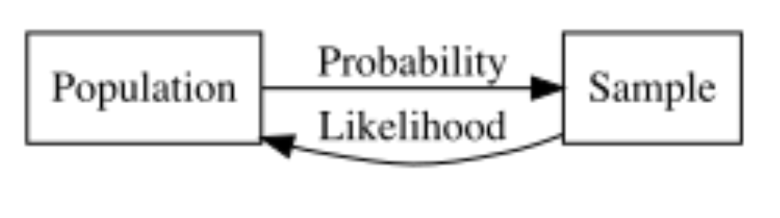
\includegraphics[width=0.5\linewidth]{Figure/Week 3/Likelihood.png}
\end{figure}

\subsubsection{Maximum Likelihood Approach}

\indent

$f(x_1,x_2,...,x_n|\theta)$ is the probability density of observing $x_1,x_2,...,x_n$ given the parameter $\theta$. Assuming independent and identically distributed variables $f(x_1,x_2,...,x_n|\theta)=\prod_{i=1}^{n}f(x_i|\theta)$, maximising the log-likelihood is often easier so it is common to maximise:

\begin{align*}
    L(\theta|x)=\prod_{i=1}^{n}f(x_i|\theta)\xrightarrow{}\mathcal{L}(\theta|x) = \ln{L(\theta|x)} = \sum_{i=1}^{n}\ln{f(x_i|\theta)}
\end{align*}

\subsection{Density Estimation - Non-parametric Approach}

\indent

Danger of misspecification with parametric approach:

\begin{itemize}
    \item If the assumed $f_\theta$ is incorrect
    \item Serious danger of inferential errors
\end{itemize}

Non-parametric approaches to density estimations:

\begin{itemize}
    \item Assume little about the structure of $f$
    \item Use local information to estimate $f$ at a point $x$
\end{itemize}

\subsubsection{Histograms}

\begin{itemize}
    \item One type of nonparametric density estimators.
    \item Piecewise constant density estimators.
    \item Very simple visualization and easy to produce.
    \item \textbf{Sensitive to the number of bins chosen and bin width}.
    \item Preferable to have a smooth estimate and not have columns.
\end{itemize}

\subsubsection{Kernel Density Estimation}

\indent

A kernel is a special type of probability density function (\textbf{PDF}) having the properties:

\begin{align*}
    & K(x)\geq 0 & \text{non-negative}\\
    & K(-x) = K(x)& \text{symmetric} \\
    & \int K(x) dx = 1 & \text{unit measure}
\end{align*}

Kernel density estimation is a non-parametric approach estimating densities. Essentially, \textbf{at every data point, a kernel function is created with the point at its centre}. The PDF is estimated by \textbf{adding all of these kernel functions and dividing by the number of data} to ensure that it satisfies:

\begin{itemize}
    \item Every possible value of the PDF is non-negative
    \item The definite integral of the PDF over its support set equals 1
\end{itemize}

\subsubsection{Kernel Density Estimator (KDE)}

\indent

A simple one weights all points within a window $h$ of $x$ equally:

\begin{align*}
    \hat{f}(x) = \frac{1}{2nh}\sum_{i=1}^{n}1_{\{|X_i-x|<h\}}
\end{align*}

\begin{align*}
\begin{cases}
    1_{A} = 1,& \text{if $A$ is true}\\
    1_{A} = 0,& \text{otherwise}
\end{cases}
\end{align*}

More generally a univariate kernel density estimator has a general weight function (Kernel):

\begin{align*}
    \hat{f}(x) = \frac{1}{nh}\sum_{i=1}^{n}K(\frac{X_i-x}{h})
\end{align*}

\begin{itemize}
    \item $K$ is a kernel function.
    \item $h$ is a bandwidth parameter (possibly fixed or varying).
    \item Consider only $h$ fixed for this course.
\end{itemize}

There are two main components for the KDE: the choice of $K$ and $h$.

\begin{itemize}
    \item The choice of Kernel is less important and generally gives similar results
    \item The choice of bandwidth is \textbf{important} and can \textbf{vary the result greatly}
\end{itemize}

Some standard kernels:

\begin{align*}
    & K(x) = \frac{1}{2}1_{\{|x|\leq 1\}} & \text{Uniform}\\
    & K(x) = \frac{1}{\sqrt{2\pi}}\exp{\{-\frac{x^2}{2}\}} & \text{Gaussian}\\
    & K(x) = \frac{3}{4}(1-x^2)1_{\{|x|\leq 1\}} & \text{Epanechnikov}
\end{align*}

\subsubsection{Choosing the Bandwidth}

\indent

The density estimator(below) is a fixed-bandwidth kernel density estimator since $h$ is constant.

\begin{align*}
    \hat{f}(x) = \frac{1}{nh}\sum_{i=1}^{n}K(\frac{X_i-x}{h})
\end{align*}

\begin{itemize}
    \item \textbf{$h$ too small}: The density estimator will tend to assign probability density too locally near observed data, causing a wiggly estimated density function with many false modes.
    \item \textbf{$h$ too large}: The density estimator will spread probability density contributions too diffusely, causing smooths away important features of $f$.
\end{itemize}

Here is a bias and variance trade-off: a small(large) bandwidth gives high variance(bias).

\subsubsection{Computing Density in R-project}

Base R-project uses command 'density', specify the bandwidth with 'bw' argument:

\begin{lstlisting}[language = R]
density.cbd <- density(x = distance.cbd, bw = 1.25, from = 0, to = 50)
summary(density.cbd)
\end{lstlisting}

\noindent Visualization:

\begin{lstlisting}[language = R]
plot(density.cbd, main = "Distance to CBD")
\end{lstlisting}

\subsection{Mean squared error, Bias, and Variance}

\indent

We can decompose the mean squared error (MSE) into the sum of three quantities: The variance, the squared bias, and the variance of the error:

Assume $Y = f(X)+\epsilon$ and we have an estimator $\hat{f}(X)$ of $f(X)$,

\begin{align*}
    \mathbb{E}(Y-\hat{f}(X))^2 = Var(\hat{f}(X))+[Bias(\hat{f}(X))]^2 + Var(\epsilon)
\end{align*}

where Bias is error introduced by approximating the data using a model.

Variance here denoting how much would $f(x)$ change if we estimate using a different training set.



\pagebreak

\section{Week 4 - High-dimensional visualisation and analytics in R}
\subsection{Unsupervised Learning}

\indent 

\noindent \textbf{Supervised Learning}:

Given a dataset with features/predictors $(X_{i1},X_{i2},...,X_{ip})$ and a target outcome variable $(Y_i)$, the goal is to learn a model $f(X_{i1},...,X_{ip})$ to explain/predict the target.

\noindent \textbf{Unsupervised learning}:

Given a dataset with features $(X_{i1},X_{i2},...,X_{ip})$, the goal is to visualise, find patterns, subgroups/clusters within the data.

\subsection{Clustering}

\subsubsection{Overview}

\indent 

\noindent\textbf{Clustering}:

Groups similar observations based on a \textbf{similarity measure}.

\noindent\textbf{Clustering Goals}:

\begin{itemize}
    \item \textbf{Compact Clusters}: Observations within a cluster should be close together.
    \item \textbf{Well-Separated Clusters}: Observations from different clusters should be far apart.
\end{itemize}

\subsubsection{Typical methods}

\noindent\textbf{Partitioning}:

\begin{itemize}
    \item Pre-specified number $K$ of mutually exclusive and exhaustive groups.
    \item Iterate until criteria is met
\end{itemize}

\noindent\textbf{Hierarchical methods}:

\begin{itemize}
    \item Agglomerative: Bottom up, more popular
    \item Divisive: Top down, less popular
    \item Display results with dendrogram
\end{itemize}

\subsubsection{$K$-Means Clustering}

\noindent\textbf{Measuring Cluster Compactness}:

For cluster $C_k$, we can define within-group sum of squares as:

\begin{align*}
    \text{WSS}_k = \frac{1}{|C_k|}\sum_{i,j\in C_k}||x_i - x_j||^2, k = 1,...,K
\end{align*}

This is the sum of all the pairwise squared Euclidean distances between observations in the $k^{th}$ cluster, divided by total number of observations in the $k^{th}$ cluster.

$\sum_{i,j \in C_k}||x_i - x_j||^2$ is the sum of all the pairwise squared Euclidean distances between observations in the $k^{th}$ cluster.

$|C_k|$ is the total number of observations in the $k^{th}$ cluster.

\bigskip

\noindent\textbf{Clustering Objective}:

To minimize the total within-group sum of squares criterion.

\begin{align*}
    \text{WSS}_{\text{Total}} = \sum_{k=1}^{K}\text{WSS}_k
\end{align*}

The total within sum of square criterion will \textbf{decrease} as $K$ increases.

Rule of thumb: Look for the elbow.

\begin{figure}[h]
    \centering
    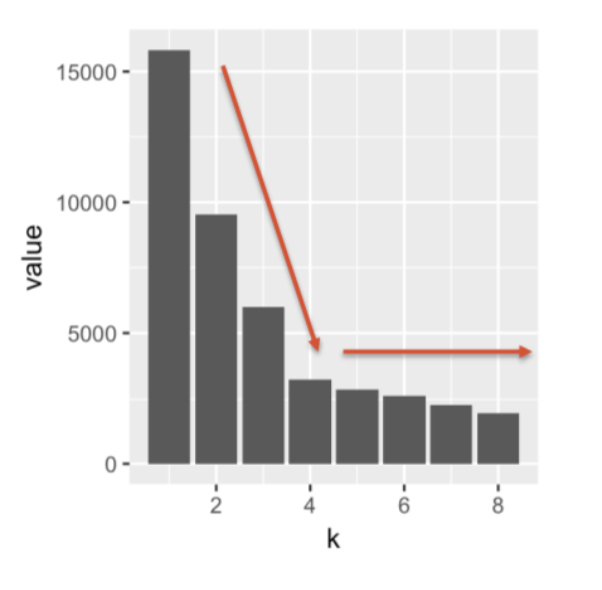
\includegraphics[width=0.5\linewidth]{Figure/Week 4/Elbow.png}
    \caption{Elbow Plot}
\end{figure}

\bigskip

\noindent\textbf{Process}:

Initialise each observation at random to a cluster.

Iterate the following until the assignments stop changing:

\begin{itemize}
    \item For each of the $K$ clusters, compute the cluster centroid.
    \item Assign each observation to the cluster whose centroid is closest (where the closest is defined using the Euclidean distance).
\end{itemize}

\bigskip 

\noindent\textbf{Properties}:

\begin{itemize}
    \item The number of clusters $K$ needs to be specified.
    \item Local solution and not necessarily global solution.
    \item Depends on starting values (the random starting values)-run the algorithms multiple times.
    \item Best for compact, spherical clusters.
    \item Does not work well when cluster sizes are different.
\end{itemize}

\subsubsection{Hierarchical clustering}

\indent 

Begin with every observation representing a single cluster.

At each iteration, merge the two closest clusters into one cluster:

\begin{itemize}
    \item Needs \textbf{a measure of similarity/dissimilarity} between two clusters
    \item These measures are called \textbf{linkages}.
\end{itemize}

\noindent\textbf{Linkages}: 

Measure of dissimilarity between two sets of objects that determine how two set of objects are merged.

\begin{itemize}
    \item Single linkage
    \item Complete linkage
    \item Average Linkage
\end{itemize}

\begin{figure}[h]
    \centering
    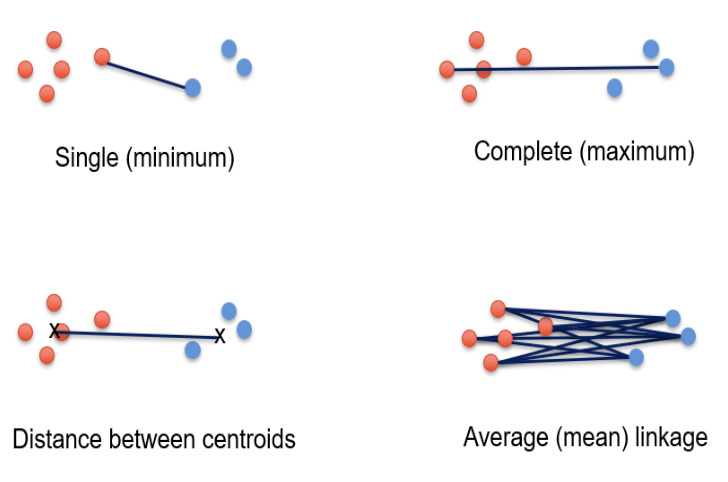
\includegraphics[width=0.8\linewidth]{Figure/Week 4/Linkages.png}
\end{figure}

\subsection{Principal Components Analysis (PCA)}

\indent 

Suppose we have a data matrix $X$ with $n$ observations and $p$ features. Principal Component Analysis (PCA) helps us reorganise/transform the data into a new coordinate system. The data still has $p$ dimensions, but in a new set of axes. The goal is to capture most of the variation using just the first few dimensions, making the data easier to analyse.

\subsubsection{High-dimensional data}

High-dimensional data refers to data set with more features $p$ than observations $n$.

It is very hard to visualize high-dimensional data. Only have 2 (sometimes 3 or 4) dimensional canvas to create plots. Many algorithms and methods have been designed for low dimensional data and would not work well for high-dimensional data.

\subsubsection{Dimension reduction strategies}

\indent 

\noindent\textbf{Eliminate or remove features}

\noindent\textbf{Select features} (Example: Lasso and ridge regression)

\noindent\textbf{Build or construct new features from existing ones}

\begin{itemize}
    \item Replace many existing features with a single one.
    \item PCA and $t$-SNE
\end{itemize}

\subsubsection{Principal components}

\indent 

\begin{figure}[h]
    \centering
    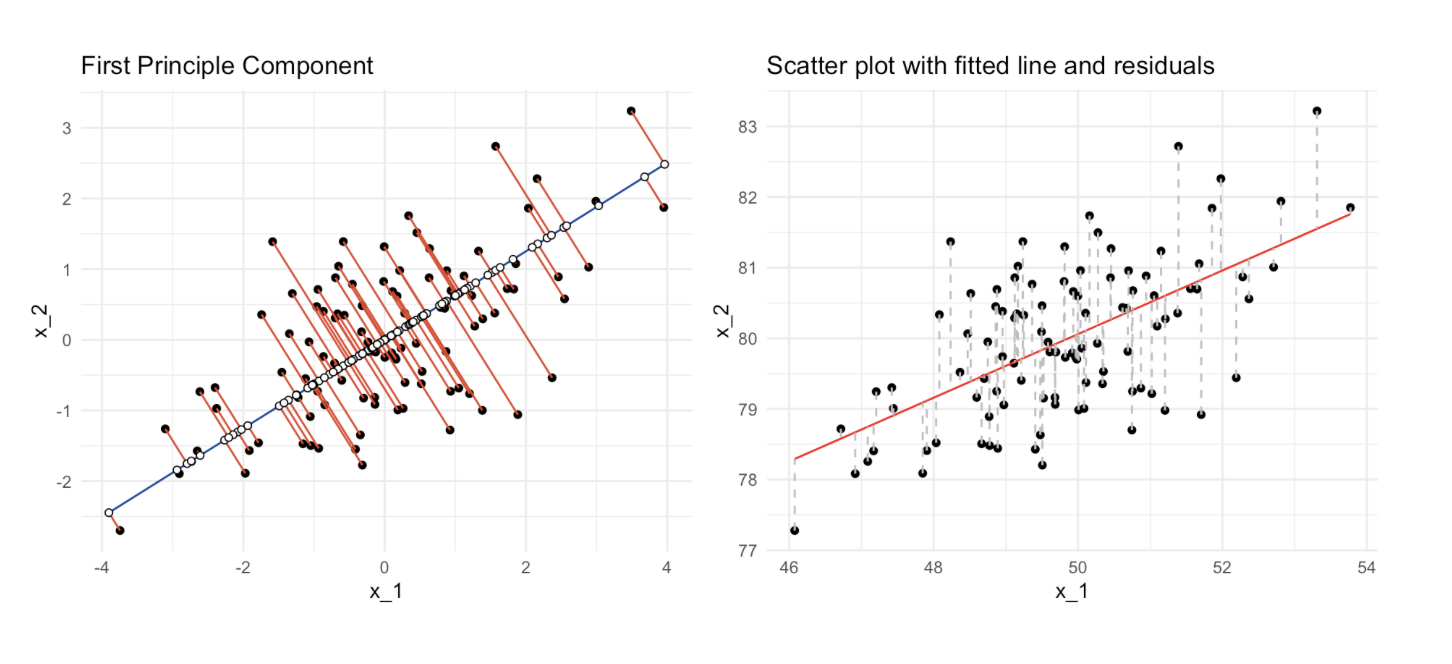
\includegraphics[width=0.8\linewidth]{Figure/Week 4/Geometric.png}
    \caption{Geometric interpretation}
\end{figure}

Start with a data matrix $\boldsymbol{X}$, and assume it has \textbf{mean zero}.

\begin{align*}
    \boldsymbol{X} = (X_1,X_2,...,X_n)
\end{align*}

The first principal component is the \textbf{normalised linear combination of the features} that \textbf{maximises the variance} in the new component.

\begin{align*}
    & Z_1 = \phi_{11}X_1+\phi_{21}X_2+...+\phi_{p1}X_p = \sum_{j=1}^{p}\phi_{j1}X_j = \boldsymbol{X}\boldsymbol{\phi}_{1}\\
    & \boldsymbol{\phi}_1 = (\phi_{11},...,\phi_{p1})^T
\end{align*}

The elements $\phi_{j1}$ are known as the loadings of the first principal component.

By normalised, we mean the squared loadings have to sum to 1:

\begin{align*}
    \sum_{j=1}^p\phi_{j1}^2 = 1 \iff \boldsymbol{\phi}_1^T\boldsymbol{\phi}_1 = 1
\end{align*}

It is desired to maximise the sample variance of $Z_{i1},...,Z_{n1}$, where $Z_{i1}$is the $i-th$ componenet of $Z_1$:

\begin{align*}
    \frac{1}{n-1}\sum_{i=1}^n(\sum_{j=1}^p\phi_{j1}x_{ij})^2
\end{align*}

Given the principal component loadings, we can project our data matrix $\boldsymbol{X}$ onto the principal component space.

\noindent\textbf{Principal component score}: The projection is a linear combination of the sample feature values.

\begin{align*}
    z_{i1} = \phi_{11}x_{i1}+\phi_{21}x_{i2}+...+\phi_{p1}x_{ip}
\end{align*}

The first principal component score vector is:

\begin{align*}
    \boldsymbol{Z}_1 = (z_{11},z_{21},...,z_{n1})
\end{align*}

The principal component score vectors are uncorrelated (orthogonal).

\subsubsection{Preprocessing for PCA}

\indent 

In PCA, it’s common to center variables by subtracting the mean. You can also standardise them so all variables have a standard deviation of 1. Standardising ensures all variables contribute equally. Improves interpretability and prevents one variable from dominating the analysis.

\noindent \textbf{Why Standardisation}: Variables may have different units. This leads to different variances, affecting PCA results.

\noindent \textbf{Impact on Loadings}: PCA loadings give more weight to variables with higher variance. This can bias the analysis if some variables dominate.

\subsubsection{PCA Properties}

\begin{itemize}
    \item Unique and Global solution!
    \item Ordered components
    \item Best linear dimension reduction possible
    \item Is not the best for non-linear relationships
\end{itemize}

\subsubsection{PCA with $K$-means}

\indent 

Very common approach to deal with high dimensional data.

Use the first $M$ principal component scores as inputs into the $K$-means algorithm, where $M\ll p$.

Can help improve the clustering model if the signal in the data can be captured in a few principal components.

\subsubsection{PCA with regression}

\indent 

Use the first $M$ principal component scores as the predictors in a linear regression model.

We are assuming that a small number of principal components can explain most of the variability in the data as well as the response.

PCA is useful when variables in the data are highly correlated (i.e., collinear).

\subsection{Dimension reduction $t$-SNE}

\indent 

Non-linear technique developed for visualizing high dimensional datasets.

Use local structure in the data to find a low dimensional representation.

\subsubsection{$t$-SNE vs PCA}

\indent 

\begin{figure}[h]
    \centering
    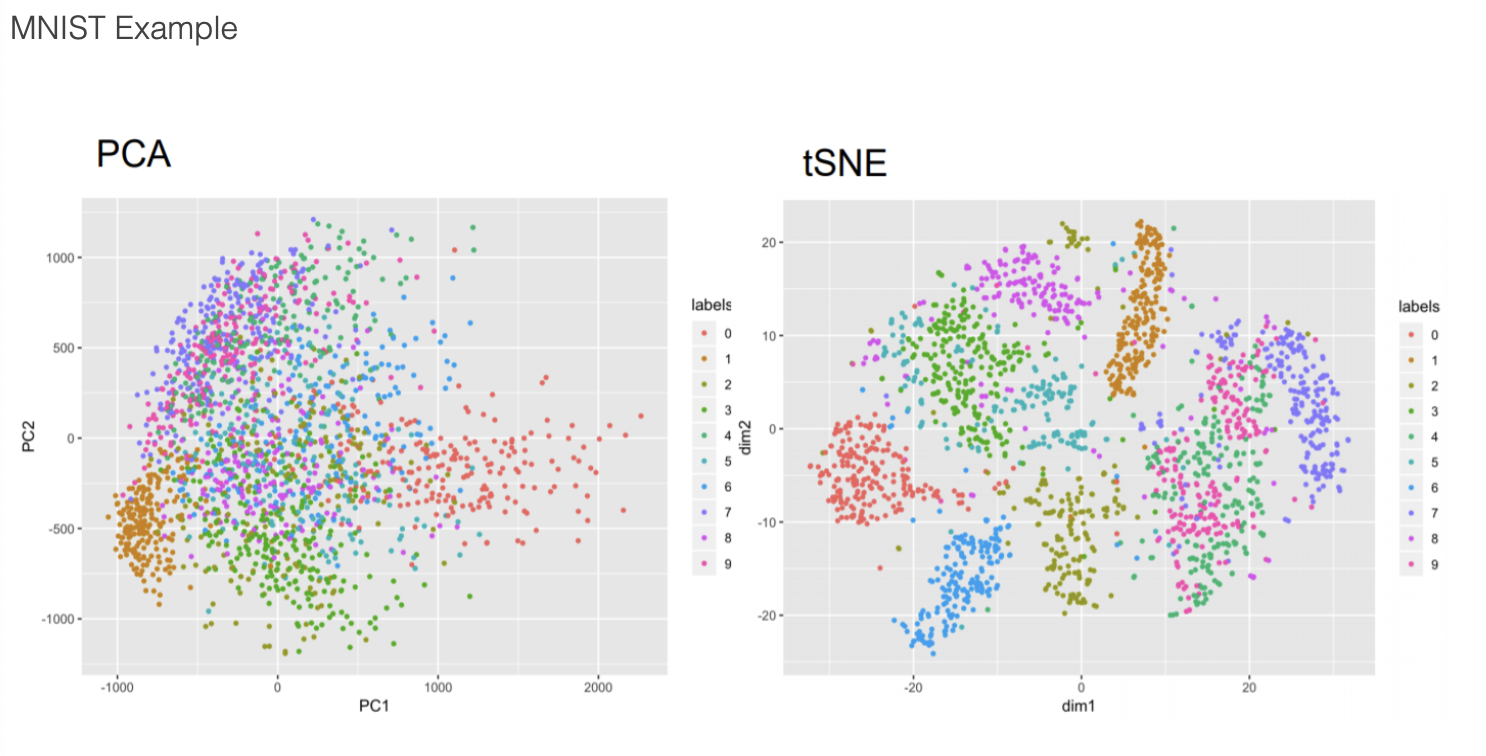
\includegraphics[width=0.8\linewidth]{Figure/Week 4/t-SNE VS PCA.png}
\end{figure}

\noindent\textbf{PCA}

\begin{itemize}
    \item PCA is a linear method and can only capture linear relationships.
    \item PCA is defined by a mathematical formula.
    \item The principal components (PCs) from PCA can be interpreted and used for inference.
    \item PCA is less computationally intensive
\end{itemize}

\noindent\textbf{$t$-SNE}

\begin{itemize}
    \item $t$-SNE is a non-linear technique and is able to find complicated non-linear relationships.
    \item $t$-SNE is a probabilistic method – it will give you a different representation every time you run it
    \item $t$-SNE is mostly a visualization method. The visualization from $t$-SNE cannot be used for inference.
    \item $t$-SNE is more computationally intensive
\end{itemize}

\subsection{Dimension reduction: Multidimensional Scaling (MDS)}

\indent 

Visually represent proximities (similarities or distances) between objects in a lower dimensional space (usually 2 or 3d space).

The objective of MDS is to take a Matrix of similarities or dissimilarities, $\boldsymbol{D}$, and find projections $z_1,...,z_k$ where $k$ is the desired lower dimension.

The distances are near preserved by optimizing a stress function.

Full data not required.

\subsubsection{MDS Stress functions}

\indent 

These functions attempt to force the lower dimensional projections to preserve the distances in the original data.

\noindent\textbf{Commoon stress functions}:

\begin{align*}
    \text{Least Squares:}S_{LS}(z_1,z_2) = \sqrt{\sum_{i\neq j}(d_{ij} - ||z_i-z_j||)^2}
\end{align*}

\subsubsection{Comments on MDS}

\indent 

\noindent\textbf{Pros \& Cons}:

\begin{itemize}
    \item Requires only a distance or dissimilarity matrix, not the full dataset.
    \item Must choose the number of dimensions KK (similar to the elbow method in a Scree plot).
    \item Useful for visualizing non-linear data in a lower-dimensional space.
\end{itemize}

\bigskip 

\noindent\textbf{How to Interpret MDS Maps}

\begin{itemize}
    \item Rotation does not matter – axes and orientation are arbitrary.
    \item Focus on relative positions – only distances between points are meaningful.
    \item Objects closer together on the MDS map are more similar based on the input distance matrix.
\end{itemize}
\pagebreak

\section{Week 5 - Classification technique}
\subsection{Mean Squared Error (MSE)}

\indent 

The MSE measures the average squared difference between the predicted values and the true values:

\begin{align*}
    \text{MSE} = \mathbb{E}[(Y-\hat{f}(X))^2]
\end{align*}

\textbf{MSE Can Be Decomposed Into Three Components:}

\begin{align*}
    \text{MSE} = \mathbb{E}[(y_0-\hat{f}(x_0))^2] = \text{Bias}^2+\text{Var}(\hat{f}(x_0))+\text{Var}(\epsilon)
\end{align*}

\subsubsection{Bias-Variance Tradeoff}

\indent

\noindent \textbf{High complexity/flexibility model}: 

\begin{itemize}
    \item \textbf{Low bias}: fits the training data well, overfits.
    \item \textbf{High variance}: sensitive to noise.
\end{itemize}

\noindent\textbf{Low complexity/flexibility model}:

\begin{itemize}
    \item \textbf{High bias}: too simple, underfits.
    \item \textbf{Low Variance}: more stable across different samples.
\end{itemize}

\subsection{Classification}

\subsubsection{Basic Principles}

\indent 

Each observation consists of class label $y$ (categotical variable) and feature vector $\boldsymbol{x} = (x_1,x_2,...,x_p)$ (mix of categorical and continuous variables).

Goal is to classify $y$ using $\boldsymbol{x}$. Classification models produce a continuous valued prediction, which is usually in the form of a probability (i.e., the predicted values of class membership for any individual sample are between 0 and 1 and sum to 1). It require a rule to assign observations to a category based on the predicted probability.

\subsubsection{Classification vs Clustering}

\indent 

\noindent\textbf{Classification}: classes are predefined, want to use a training set of labeled objects to form a classifier for classification of future observations (supervised)

\noindent\textbf{Clustering}: classes are unknown, want to discover them from the data (unsupervised)

\subsubsection{Two class classification (Binary)}

\indent 

Binary in there are two possible values (0 or 1, TRUE or FALSE).

\noindent\textbf{Linear regression misspecifications}: The regression line $\beta_0+\beta_1x$ can span the entire real line, all values between $-\infty$ to $+\infty$. For the target variable $y$ only takes two values: 0 or 1, the linear regression model is not well specified for this purpose.

\subsection{Logistic regression}

\indent 

The multiple regression could write as $\mathbb{E}[Y|X] = \boldsymbol{X\beta}$.

\begin{align*}
    Y & = \boldsymbol{X\beta}+\epsilon\\
     & = \beta_0 + \beta_1X_1+...+\beta_pX_p+\epsilon
\end{align*}

This can generalise this to $g(\mathbb{E}[Y|X]) = \boldsymbol{X\beta}$.

Logistic regression is a special case of one of these generalised linear models:

\begin{align*}
    \log(\frac{p}{1-p}) = \boldsymbol{X\beta}, p = P(Y=1|X)
\end{align*}

Dolve for $p$ gives:

\begin{align*}
    p = g^{-1}(\boldsymbol{X\beta}) = \frac{1}{1+\exp{(-\boldsymbol{X\beta})}}
\end{align*}

\subsubsection{Terminology}

Logistic function responsible from mapping the features from $(-\infty,+\infty) = \mathbb{R}$ to $(0,1)$.

we want the values in the logit space to be linear in $\boldsymbol{X}$, We choose 
$\beta$ that minimizes the negative log-likelihood (log-loss):

\begin{align*}
    \ell(\beta) = \sum_{i=1}^n -y_i\log(p(x_i)) - (1-y_i)\log(1-p(x_i))
\end{align*}

Gradient-descent methods can be used for optimization.

Decision boundary: predict $Y=1$ if $\boldsymbol{X\beta}\geq 0$.

\subsection{Linear Discriminant Analysis (LDA)}

\indent 

LDA classifies data by finding the decision boundary that best separates different classes, assuming the data follows Gaussian distributions with a class specific mean $(\mu_k)$ and a common variance $(\sigma^2)$.

\subsubsection{Bayes’ Theorem in the classification context}

\begin{align*}
    p_k(x) = P(Y=k|X=x) = \frac{\pi_kf_k(x)}{\sum_{i=1}^K\pi_\ell f_\ell (x)}
\end{align*}

$f_k(x)$ is the density function for feature $x$ given it’s in group $k$.

\begin{itemize}
    \item Posterior: The probability of classifying observation to group $k$ given it has features $x$.
    \item Prior: The prior probability of an observation in general belonging to group $k$
\end{itemize}

\subsubsection{LDA setup}

\indent 

Using the Bayes’ Theorem, we model:

\begin{align*}
    & p_k(x) = P(Y=k|X=x) = \frac{\pi_kf_k(x)}{\sum_{i=1}^K\pi_\ell f_\ell (x)}\\
    & \pi_k: \text{Probability of coming from class $k$ (prior probability)}\\
    & f_k(x): \text{Density function for $X$ given that $X$ is an observation from class $k$}
\end{align*}

This is a generative approach that models the distribution of each class (assuming Gaussian distributions) and then uses Bayes’ theorem to find the decision boundary.

\subsubsection{Estimation of $\pi_k$ and $f_k(x)$}

\indent 

We can estimate $\pi_k$ and $f_k(x)$ to compute $p_k(x)$. The most common model for $f_k(x)$ is the Normal Density $N(\mu_k,\sigma_k^2)$.

If we use the above density, we only need to estimate $3$ quantities to compute $p_k(x)$: $\mu_k, \sigma_k^2, \pi_k$.

For simplicity, we assume common variance $\sigma = \sigma_1 = ...=\sigma_k = ...$.

We can allow the observations in the $k$-th class to have a class-specific variance $\sigma_k^2$, leading to the quadratic discriminant analysis.

\begin{itemize}
    \item The mean $\mu_k$ could be estimated by the average of all training observations from the $k$-th class.
    \item The variance $\sigma^2$ could be estimated as the weighted average of variances of all $K$ classes.
    \item The poportion $\pi_k$ could be estimated as the proportion of the training observations that belong to the $k$-th class.
\end{itemize}

Here, $n $ is the sample size, $n_k$ is the number of samples in the $k$-th class.

\begin{align*}
    & \hat{\mu}_k = \frac{1}{n_k}\sum_{i:y_i = k}x_i\\
    & \hat{\sigma}^2 = \frac{1}{n-K}\sum_{k=1}^K\sum_{i:y_i = k}(x_i - \hat{\mu}_k)^2\\
    & \hat{\pi}_k = \frac{n_k}{n}
\end{align*}

\subsubsection{Why LDA?}

\indent 

In the case where \textbf{$n$ is small, and the distribution of predictors $X$ is approximately normal}, then LDA is more stable than Logistic Regression. 

LDA is more popular when we have \textbf{more than two response classes}. More intuitive to predict class assignment. But logistic regression CAN be generalised for classification problems with more than two classes.

When classes are \textbf{perfectly separated}, the parameter estimates in logistic regression become infinite. This can lead to instability in software (e.g., R) when estimating parameters. In contrast, LDA remains stable and does not face this issue.

LDA may perform poorly for categorical predictors due to the normality assumption.

\subsubsection{Logistic Regression vs LDA}

\indent 

\noindent\textbf{Similarity:}

Both Logistic Regression and LDA produce \textbf{linear boundaries}.

\bigskip

\noindent\textbf{Differences:}

\begin{itemize}
    \item LDA assumes that the observations are drawn from the normal distribution with common variance in each class, while logistic regression does not have this assumption.
    \item LDA would do better than Logistic Regression if the assumption of normality hold, otherwise logistic regression may outperform LDA
\end{itemize}

\subsection{$k$-Nearest Neighbours (kNN)}

\indent 

The kNN model computes the probability of an observation with features $x$ belonging to group $\ell$ based on the membership of the nearest points (denoted by $N_x^k)$ to $x$.

\begin{align*}
    P(Y = \ell|x) = \frac{1}{k}\sum_{i\in N_x^k}1_{\{y_i = \ell\}}
\end{align*}

Here $\sum_{i\in N_x^k}1_{\{y_i = \ell\}}$ counts of the closest $k$ points that belong to group $\ell$.

\subsubsection{kNN vs LDA and Logistic Regression}

\indent 

kNN is \textbf{completely non-parametric}: No assumptions are made about the shape of the decision boundary.

\noindent \textbf{Advantage}:

We can expect kNN to dominate both LDA and Logistic Regression when the decision boundary is highly non-linear.

\bigskip

\noindent\textbf{Disadvantage}:

\begin{itemize}
    \item kNN does not tell us which predictors are important (no table of coefficients).
    \item The choice of the number of $K$ matters.
\end{itemize}

\subsection{Support Vector Machines (SVM)}

\indent 

SVM finds a decision boundary (hyperplane) that best separates the two classes by maximising the margin between them.

\textbf{Support vectors}: observations that either lie on or violate the margin

\subsubsection{Hyperplane}

\indent 

In $p$ dimensions, it is a flat affine subspace of dimension $p-1$.

For the general equation: $\beta_0 + \beta_1X_1+...+\beta_pX_p = 0$. If $\beta_0=0$, the hyperplane passes through the origin, otherwise it does not. The vector $(\beta_1,\beta_2,...,\beta_p)$ is called the normal vector - It points in a direction orthogonal to the surface of the hyperplane.

\subsubsection{Separating hyperplanes}

\begin{figure}[h]
    \centering
    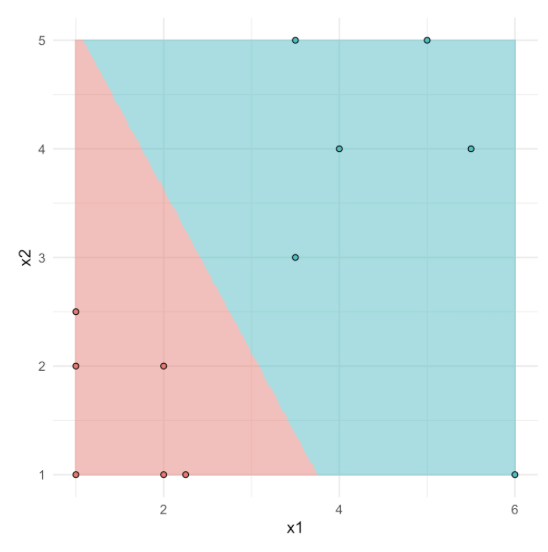
\includegraphics[width=0.5\linewidth]{Figure/Week 5/Separating hyperplanes.png}
\end{figure}

Consider coding Red as $y_i=-1$ and blue as $y_i=1$, then $y_if(x_i)>0$ for all $i$, $f(x_i)$ defines a separating hyperplane.

If $f(x_i) = \beta_0 + \beta_1X_1+...+\beta_pX_p$ defines a hyperplane, $f(x)>0$ defines a region on one side of the hyperplane, $f(x)<0$ defines another.

\subsubsection{Margin}

\indent 

\noindent\textbf{Maximal Margin Classifier}:

\begin{align*}
    \max_{\beta_0,...,\beta_p} M \text{ such that} &\sum_{j=1}^p\beta_j^2 = 1\\
    & y_i(\beta_0+\beta_1x_{i1}+...+\beta_px_{ip})\geq M, i = 1,...,n
\end{align*}

\bigskip

\noindent\textbf{Soft margin}:

\begin{figure}[h]
    \centering
    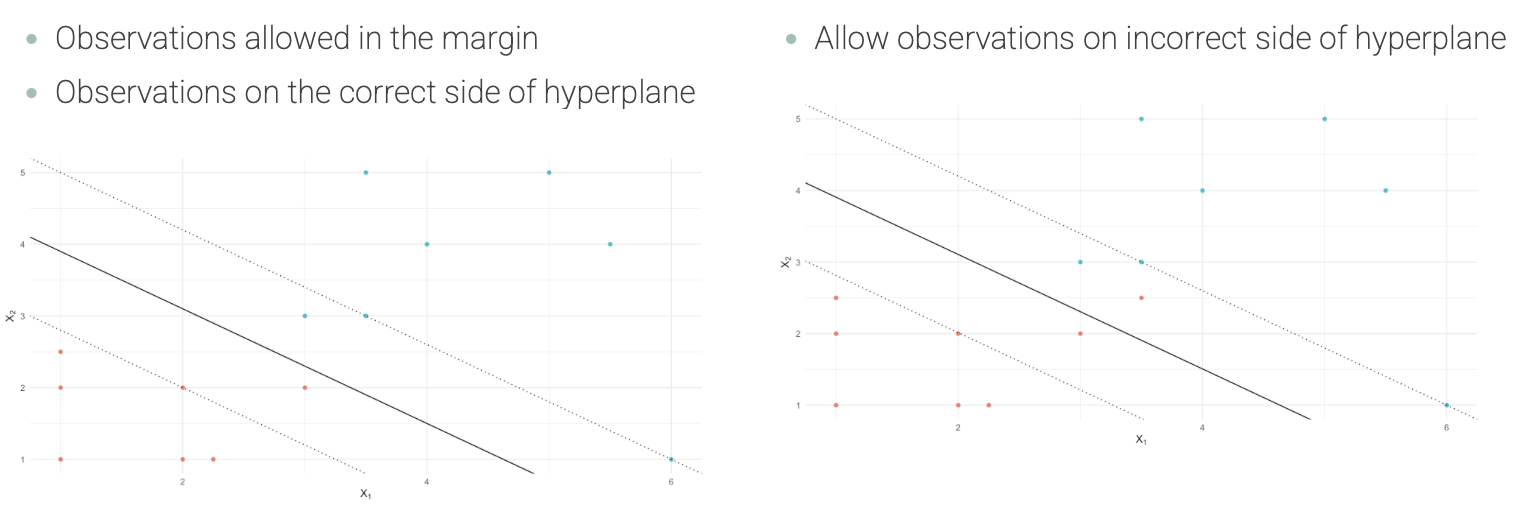
\includegraphics[width=0.8\linewidth]{Figure/Week 5/Soft margin.png}
\end{figure}

If a basic mathematical plane is not possible due to non-perfect separation or outliers, we introduce a soft margin to relax the requirement for all observations to be on the correct side of the margin.

\subsubsection{Support Vector Classifier}

\indent 

Support Vector Classifier solves the following optimization problem:

\begin{align*}
    \max_{\beta_0,...,\beta_p,\epsilon_1,...,\epsilon_n}M \text{ such that } & \sum_{j=1}^p \beta_j^2 = 1\\
    & y_i(\beta_0+\beta_1x_{i1}+...+\beta_px_{ip})\geq M(1-\epsilon_i), i =1,...,n\\
    & \epsilon_i \geq0, i = 1,...,n, \sum_{i=1}^n\epsilon_i\leq C
\end{align*}

Here:

\begin{itemize}
    \item $C$ is a non-negative tuning parameter.
    \item $M$ is the width of the margin.
    \item $\epsilon_i$ are slack variables that allow observations to be on the wrong side of the margin.
    \begin{itemize}
        \item if $\epsilon_i>1$, then observation $i$ is on the wrong side of the hyperplane
        \item if $0<\epsilon_i\leq 1$, then observation $i$ is on the correct side but inside margin
        \item if $\epsilon_i = 0$, then observation $i$ is on the correct side and past the margin
    \end{itemize}
\end{itemize}

\subsubsection{Feature space expansion}

\indent 

Enlarge the space of features by including transformations:

\begin{itemize}
    \item new features that are powers and products $X_1^2,X_1^3,X_1X_2$
    \item Hence go from $p$-dimensional space to $P>p$ dimensional
\end{itemize}

Fit (linear) support vector classifier in the expanded feature space. Impact is a non-linear decision boundary in original feature space. This leads to non-linear decision boundary in the original space (quadratic conic sections).

For example, Suppose we start off in 2-dimensional feature space $(X_1,X_2)$. We make new feature space $(X_1,X_2,X_1^2,X_2^2,X_1X_2)$. Then the decision boundary would be of the form: $\beta_0+\beta_1X_1+\beta_2X_2+\beta_3X_1^2+\beta_4X_2^2+\beta_5X_1X_2 = 0$.

\subsubsection{Non-linearity and kernels}

\indent 

Polynomials add complexity and scale poorly in high dimensions. Kernels allow us to introduce non-linearity efficiently without explicitly adding features. The inner product trick enables the SVCs to classify non-linear data in an elegant and computationally efficient way.

\subsubsection{Inner products and support vectors}

\indent 

Recall $\boldsymbol{x}_i = (x_{i1},x_{i2},...,x_{ip})\in\mathbb{R}^p$.

Inner product between vectors given by:

\begin{align*}
    \langle \boldsymbol{x_i},\boldsymbol{x_j}\rangle = \sum_{k=1}^px_{ik}x_{jk}
\end{align*}

Recall the hyperplane equation $f(x) = \beta_0+\beta_1x_1+...+\beta_px_p$.

The linear support vector classifier can be represented as:

\begin{align*}
    f(x) = \beta_0+\sum_{i=1}^n \alpha_i\langle \boldsymbol{x},\boldsymbol{x_i}\rangle
\end{align*}

\subsubsection{Support set}

\indent 

The parameters $\alpha_1,\alpha_2,...,\alpha_n$ and $\beta_0$ are estimated based on the inner products between pairs of training observations.

$\hat{\alpha}_i$is non-zero only for the support points $x_i$ (i.e., ones that lie on the margin), otherwise it equals to zero.

\begin{align*}
    f(x) = \beta_0+\sum_{j\in S}\alpha_j\langle\boldsymbol{x},\boldsymbol{x_i}\rangle
\end{align*}

Here, $S$ is the support set of indices such that $\alpha_i>0$

\subsubsection{Kernel functions}

\indent 

Suppose now we replace the inner product with a generalized function of the form $K(\boldsymbol{x}_i,\boldsymbol{x}_j)$. This function is called a kernel.

In this context, the kernel quantifies the similarity of two observations:

\begin{align*}
    &\text{Polynomial kernel} & K(\boldsymbol{x}_i,\boldsymbol{x}_j) = (1+\langle\boldsymbol{x}_i,\boldsymbol{x}_j\rangle)^d\\
    &\text{Gaussian radial kernel} & K(\boldsymbol{x}_i,\boldsymbol{x}_j) = \exp(-\gamma\sum_{k=1}^p(x_{ik}-x_{jk})^2)
\end{align*}

\subsubsection{SVM with more than two classes}

\indent 

SVM covered previously are design for binary classification. To expand this to $K$ classes there are two options.

\bigskip

\noindent\textbf{One vs all}:

Fit $K$ different binary classfiers, $f_k(x)$ for $k=1,2,...,K$ where each boundary attempts to separate class $k$ vs the rest.

Then $x_i$ is classified to $k^*$ where $f_{k^x}(x_i)>f_j(x_i)$ for all $j\neq k^*$ (i.e., the largest distance from the boundary).

\bigskip

\noindent\textbf{One vs one}:

Fit all $\binom{K}{2}$ pairwise classifiers. 

Fit $x_i$ to the class that wins the most pairwise comparisons.

\bigskip

\noindent Which to use?

If $K$ is small, do one vs one. Otherwise recommended one vs all.
\pagebreak

\section{Week 6 - Cross Validation}
\subsection{Resampling Methods}

\noindent \textbf{Resampling methods}: techniques that involve repeatedly drawing samples from a training data and refitting the model on each (re)sample in order to obtain additional information about the fitted model.

\noindent Two Main Resampling Methods:

\begin{itemize}
    \item \textbf{Cross-Validation (CV)}: Used to estimate test error and select tuning parameters.
    \item \textbf{Bootstrap}: Used primarily to assess variability, e.g., standard errors and confidence intervals
\end{itemize}

\subsubsection{Training error VS test error}

\indent 

\noindent\textbf{Training error}: the performance metric applied to the observations used to train the model.

\noindent\textbf{Test error}: the average error when applying a model to predict the response on new (test) observations that were not used in the training of the model.

\bigskip

Training error is usually very different in magnitude to the test error. Training error can underestimate the test error.

\subsubsection{Test set approach}

\indent 

\step Here, we randomly divide the available set of samples into two: a training set and a test set.

\step The model is fit on the training set, and the fitted model is used to predict the responses for the observations in the test set.

\step The resulting test-set error provides an estimate of the test error.

Typically assessed using:

\begin{itemize}
    \item \textbf{MSE}: in the case of a quantitative response (regression)
    \item \textbf{Misclassification rate}: in the case of a qualitative (discrete) response (classification)
\end{itemize}

The estimate of the test error can be highly variable, depending on precisely which observations are included in the training set and which observations are included in the test set.

In the test set approach, only a subset of the observations are used to fit the model. This suggests that the test set error may tend to overestimate the test error for the model fit on the entire data set.

\subsection{$k$-fold and repeated cross validation}

\subsubsection{$k$-fold cross validation}

\indent 

Widely used approach for estimating test error. Estimates can be used to select best model, and to give an idea of the test error of the final chosen model.

randomly divide the data into $k$ equal-sized parts and the procedure is repeated $k$ times. Each time, the first fold is treated as a test set, and the method is fit on the remaining $k-1$ folds. The $\text{MSE}_i$ is computed at each iteration. The $k$-fold CV estimate is computed by averaging these values:

\begin{align*}
    \text{CV}_{(k)} = \frac{1}{k}\sum_{i=1}^{k}\text{MSE}_i
\end{align*}

\subsubsection{Repeated Cross Validation}

\indent 

It repeats the $k$-fold CV process multiple times, each with different random splits. This helps to: provide a less biased CV test error estimate. provide the variance of the CV error. It comes with a \textbf{computational cost}.

\noindent\textbf{Other things you should do it within with CV loop}:

\begin{itemize}
    \item Feature selection
    \item Hyperparameter optimization
    \item Missing data imputation
\end{itemize}

\subsubsection{Model Selection}

\indent 

The reason for doing cross-validation is to evaluate the different models by estimating their performance on unseen data. If you need to choose between kNN, LDA, logistic regression, and SVM, then you can run each of these classification algorithms with cross-validation, and pick the one with the highest CV accuracy. But then, you can go back to use all the data to build a final model.

\subsection{Classification evaluation metrics}

\subsubsection{Confusion Matrix}

\begin{figure}[h]
    \centering
    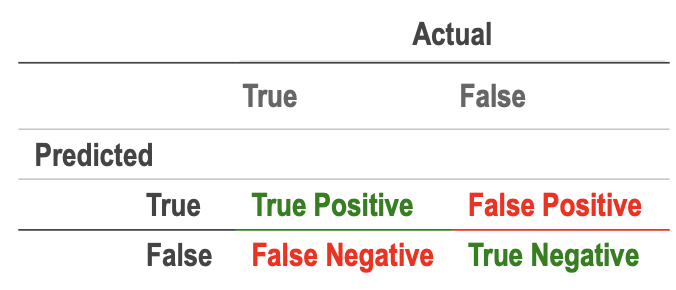
\includegraphics[width=0.6\linewidth]{Figure/Week 6/Confusion Matrix.png}
\end{figure}

\begin{itemize}
    \item \textbf{True positive}: positive class and predicted to be positive class.
    \item \textbf{False positive}: negative class but predicted to be positive class.
    \item \textbf{False negative}: positive class but predicted to be negative class.
    \item \textbf{True negative}: negative class and predicted to be negative class.
\end{itemize}

\subsubsection{Accuracy}

\begin{align*}
    \text{Accuracy} = \frac{\text{Number of Correct Predictions}}{\text{Total Number of Observations}} = \frac{TP+TN}{TP+TN+FP+FN}
\end{align*}

\noindent\textbf{Limitations of Accuracy}:

Ignores the type of error: Accuracy makes no distinction about the type of errors being made. In some cases, errors have unequal costs.

Not suitable for imbalanced data: If one class is dominant, predicting the majority class yields high accuracy but poor real performance.

\subsubsection{Alternatives}

\begin{align*}
    \text{Racall (Sensitivity)} & = \frac{TP}{TP+FN} = \frac{TP}{P}\\
    \text{Specificity} & = \frac{TN}{TN+FP} = \frac{TN}{N}\\
    \text{Precision} & =\frac{TP}{TP+FP}\\
    \text{F1} & = \frac{2\times\text{Precision}\times\text{Recall}}{\text{Precision}+\text{Recall}}\text{(Harmonic mean)}\\
    \text{GM} & =\sqrt{\text{Precision} \times \text{Recall}}\text{(Geometric mean)}
\end{align*}

\subsubsection{Receiver Operating Characteristic (ROC) Curve}

\indent 

\noindent\textbf{ROC curve}: a graphical tool used to evaluate the performance of a binary classifier.

It plots the Sensitivity against the False Positive Rate (1 - Specificity) at various threshold settings. Each point on the ROC curve corresponds to a different decision threshold. The closer the curve is to the top-left corner, the better the model.

It helps compare classification models. Useful when classes are imbalanced.

\noindent \textbf{Area Under the Curve (AUC)}: summarises the overall performance.

\begin{itemize}
    \item \textbf{$\text{AUC} = 1$}: Perfect model
    \item \textbf{$\text{AUC} = 0.5$}: No better than random guessing
\end{itemize}

\subsection{Multi-class classfication}

\indent 

Performance measured like precision, recall, $\text{F1}$, and AUC may be generalised to classification problems with more than 2 labels.
\pagebreak

\section{Week 7 - Bootstrapping, missing data, and class imbalance}
\subsection{Bootstrap}

\indent 

The bootstrap is a flexible and powerful statistical tool that can be used to quantify the uncertainty associated with a given estimator or statistical learning method.

\subsubsection{Simple example}

\indent 

Suppose that we wish to invest a fixed sum of money in two financial assets that yield returns of $X$ and $Y$ where $X$ and $Y$ are random quantities.

The goal is to create a portfolio by investing fraction $\alpha$ of our wealth in $X$ and $(1-\alpha)$ in $Y$.

Want to choose to minimise the total risk of the investment. Mathematically, this involves minimising the variance of our investment portfolio $\text{Var}(\alpha X+(1-\alpha)Y)$.

The solution to this problem (via calculus) is:

\begin{align*}
    \alpha = \frac{\sigma_Y^2 -\sigma_{XY}}{\sigma_X^2+\sigma_Y^2 - 2\sigma_{XY}}
\end{align*}

where $\sigma_X^2 = \text{Var}(X)$, $\sigma_Y^2 = \text{Var}(Y)$, $\sigma_{XY}^2 = \text{Cov}(X,Y)$.

\subsubsection{Experiment}

\indent

The values of $\sigma_X^2,\sigma_Y^2$, and $\sigma_{XY}$ are unknown but estimates can be computed from the data.

The estimate of $\alpha$ that minimises the variance of the investment can then be computed with

\begin{align*}
    \widehat{\alpha} = \frac{\widehat{\sigma}_Y^2 -\widehat{\sigma}_{XY}}{\widehat{\sigma}_X^2+\widehat{\sigma}_Y^2 - 2\widehat{\sigma}_{XY}}
\end{align*}

Suppose that $X$ and $Y$ can be sampled from the population repeatedly. 

You sample 100 pairs of $(X,Y)$ from the population — this gives you one dataset. You calculate an estimate, say $\widehat{\alpha}$, from this sample. Now, repeat this sampling process 1000 times, each time drawing a new random sample of 100 pairs from the population and computing $\widehat{\alpha}$. You will end up with $\widehat{\alpha}_1,...,\widehat{\alpha}_{1000}$.

\bigskip

Consider the mean of all the parameter estimates $\bar{\widehat{\alpha}} = \frac{1}{1000}\sum_{k=1}^{1000} \widehat{\alpha}_k$, this is close to the true value.

Estimate of the standard error using the standard deviation of all the estimates $\sqrt{\frac{1}{1000-1}\sum_{k=1}^{1000}(\widehat{\alpha}_k - \bar{\widehat{\alpha}})^2}$.

This gives an intuitive description of the reliability of the estimator. For a random sample the estimate would vary around the true value.

\subsubsection{Sampling Variability and the Variance of an Estimator}

\indent 

When we estimate a parameter, the result depends on the sample. If we collecte a different sample, the estimate would likely be different. This phenomenon is called \textbf{sampling variability}.

The variance of an estimator captures this variability: If an estimator has low variance, repeated samples yield similar results. If it has high variance, the estimate fluctuates a lot between samples.

Ideally, we want estimators that are: \textbf{Unbiased} (on average, close to the true value), \textbf{Low variance} (stable across samples).

Estimating the variance of an estimator requires repeatedly sample from the population.

\subsubsection{Application in Reality}

\indent 

We can’t actually sample repeatedly from the population. In reality, we only have one dataset, not the entire population to draw from.

\textbf{Bootstrap attempts to mimic this process}. Instead of sampling new independent observations from the population. Re-sample observations from the data with replacement. Some observations may appear more than once while others not at all.

\subsection{Missing Values}

\subsubsection{Missing Mechanisms}

\indent 

\noindent \textbf{Missing Completely at Random (MCAR)}:

Missingness has no association with any data you have observed, or not observed. Missingness occurs \textbf{purely by chance}.

Handling: Imputation is advisable. Deleting observations will not bias the results, but may reduce the model power due to the reduced sample size thus limiting inference.

\bigskip

\noindent\textbf{Missing at Random (MAR)}

Missingness depends on \textbf{data observed}, but not data unobserved.

Handling: Use imputation to adjust for missing data.

\bigskip

\noindent\textbf{Missing Not at Random (MNAR)}

Missingness is related to unobserved data.

Handling: Requires modeling the missingness mechanism to correct biases.

\subsubsection{Identifying different types of missingness}

\indent 

It’s often difficult to determine the missingness mechanism using statistical tests alone.

Instead, rely on:

\begin{itemize}
    \item \textbf{Domain knowledge} and understanding of the \textbf{data collection process}.
    \item \textbf{Predictive models}: Fit a classification model to predict missingness—if successful, data may be MAR.
\end{itemize}

For testing MCAR:

\begin{itemize}
    \item Use tests like mcar\_test() from the naniar package.
    \item Based on Little’s MCAR test (Little, 1988), which assumes multivariate normality.
\end{itemize}

\subsubsection{Dealing with missing values}

\indent 

For categorical data, “missing” can be a category.

Delete data with missing value. Two options:

\begin{itemize}
    \item Omit the variable with missing data
    \item Omit the observation with missing data
\end{itemize}

Drawbacks are that you might be throwing away valuable information, or inadvertently introduce bias into the data.

\textbf{Impute: fill in the missingness}.

\subsubsection{Imputation}

\indent 

\noindent\textbf{Single imputation}

Single imputation replaces the missing value with a single value.

\textbf{Drawbacks}: With single imputation, once the missing data are added back, it is treated as valid observed data, hence the uncertainty in the missing value data is lost.

\bigskip

\noindent\textbf{Multiple imputation}

Multiple imputation accounts for uncertainty in the imputation process
Generally follows three steps:

\step Impute the data $k$ times (this can be done using a single imputation method).

\step Perform analysis (e.g., regression/classification) on each of the $k$ imputed data sets.

\step Pool the $k$ results together

Multiple Imputation by Chained Equation (MICE) is a popular method.

\subsubsection{Other practical suggestions}

\indent 

It is highly recommend that you visualize your data to look for patterns of missingness.

Be wary of variables with high proportion of missing data. However, this might not be a problem if imputation is applicable and performs well.

Some algorithms can cope with missingness (e.g., decision trees) and so you may not need to do imputation.

If you believe the pattern of missingness is informative, you can include it as a dummy variable.

\subsubsection{R packages for dealing with missing values}

\begin{itemize}
    \item Impute (Bioconductor package): KNN imputation, written for microarray data.
    \item MICE: Multiple imputation.
    \item missForest: Uses Random Forest (in upcoming tree-based module) to predict the missing values. Can be used for continuous and categorical data.
    \item Amelia II: Multiple imputation.
\end{itemize}

\subsection{Class Imbalance}

\indent 

Example: Let’s say we have a classification problem to detect credit card fraud, but only 1\% of transactions are fraud. If you use accuracy as the metric to optimise, then just classifying every transaction as not-fraud will get you to 99\% accuracy!

\subsubsection{Cohen’s Kappa}

\indent 

\begin{align*}
    \kappa = \frac{P_o - P_e}{1-P_e}
\end{align*}

where $P_o$ is observed accuracy, $P_e$ is expected accuracy generated simply by chance.

\bigskip

\noindent\textbf{Interpretation Guide}

\begin{table}[h]
\centering
\begin{tabular}{|c|c|}
\hline
\textbf{Kappa Value} & \textbf{Strength of Agreement} \\ \hline
\textless 0          & Less than chance               \\ \hline
0.01–0.20            & Slight                         \\ \hline
0.21–0.40            & Fair                           \\ \hline
0.41–0.60            & Moderate                       \\ \hline
0.61–0.80            & Substantial                    \\ \hline
0.81–1.00            & Almost perfect                 \\ \hline
\end{tabular}
\end{table}

\subsubsection{Handelling Class Imbalance}

\indent 

\begin{itemize}
    \item Use different metrics
        \begin{itemize}
            \item $F_1$ Score:
            \begin{align*}
                F_1 = \frac{2\text{TP}}{2\text{TP}+\text{FP}+\text{FN}} = \frac{2\times \text{Precision}\times \text{Recall}}{\text{Precision}\times \text{Recall}}
            \end{align*}
            \item Area Under Curve (AUC) for the ROC
            \item Cohen’s Kappa
    \end{itemize}
    \item Modify the Data
\end{itemize}

\bigskip

\begin{figure}[h]
    \centering
    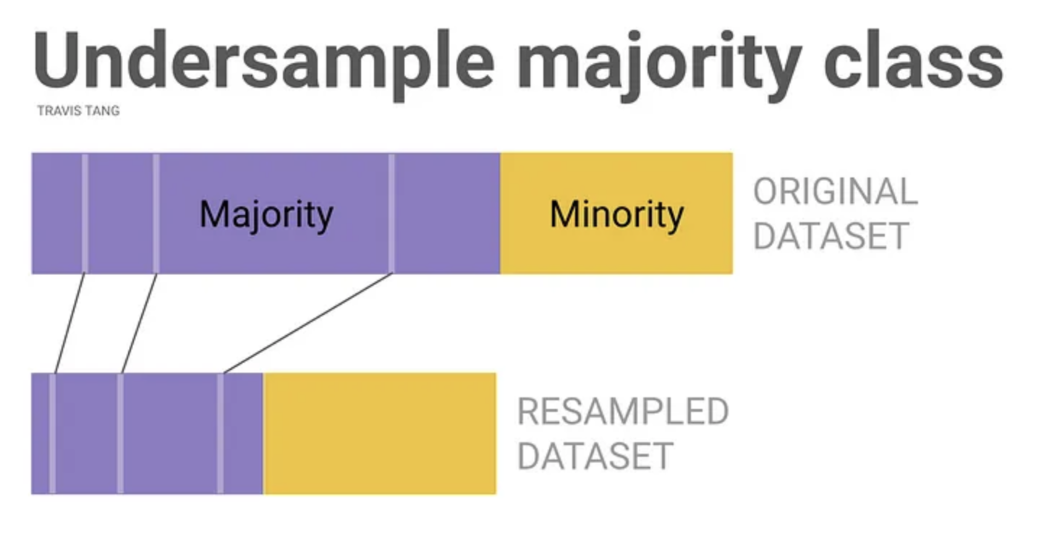
\includegraphics[width=0.8\linewidth]{Figure/Week 7/Down-sampling.png}
    \caption{Down-sampling}
\end{figure}

\noindent\textbf{Down-sampling}

Advantage: it does not introduce duplicates and/or artificial instances.

Disadvantages:

\begin{itemize}
    \item Not all data points are used.
    \item Potentially removing useful information.
\end{itemize}

Better choice for data with very high class imbalance.

\bigskip

\begin{figure}[h]
    \centering
    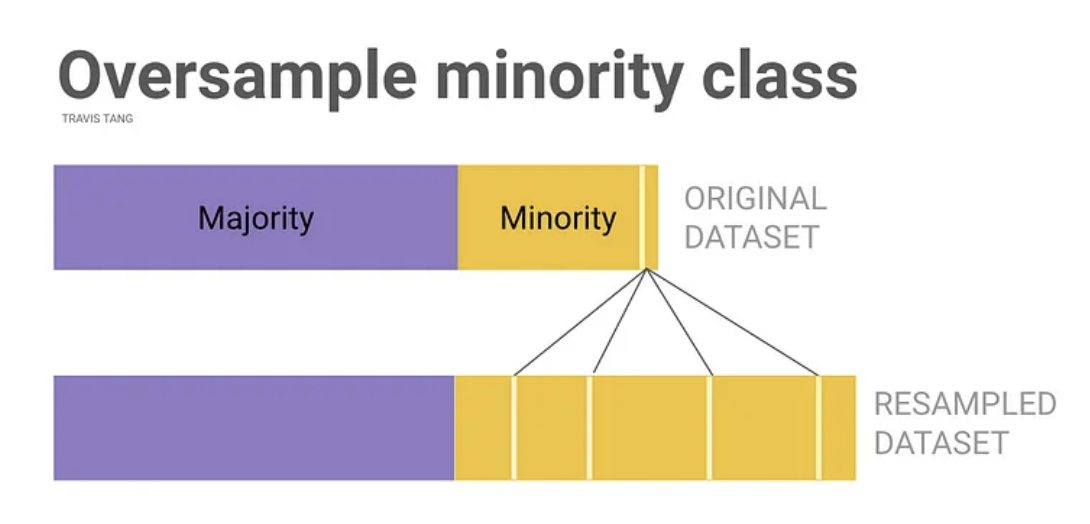
\includegraphics[width=0.8\linewidth]{Figure/Week 7/Up-sampling.png}
    \caption{Up-sampling}
\end{figure}

\noindent\textbf{Up-sampling}

Random up-sampling

Disadvantages:

\begin{itemize}
    \item creates duplicated and/or artificial instances
    \item can introduce bias and/or noise to the original data
\end{itemize}

\subsubsection{Create synthetic samples of the minority class}

\indent 

\textbf{Synthetic Minority Over-sampling Technique (SMOTE)} is a popular algorithm.

It creates synthetic samples from the minority class by:

\step Finding the $k$-nearest-neighbours for minority class observations.

\step Randomly choosing one of the $k$-nearest-neighbours, then using it to create a similar but random new observation.

Be careful that you split your data into training/test sets before doing any oversample/SMOTE. Otherwise, you will leak information from training to test data set.
\pagebreak

\section{Week 8 - Feature Selection}
\subsection{Feature Selection - Searching}

\subsubsection{Goals of feature selection}

\indent 

\textbf{Prediction accuracy}: especially when $p\geq n$. $p$ is the number of features, and $n$ is the number of observations.

\textbf{Model interpretability}: Removing irrelevant or poor features (that is, by setting the corresponding coefficient estimates to zero) $\xrightarrow{}$ we can obtain a model that is more easily interpreted.

Some approaches for feature selection are presented.

\subsubsection{Approaches for feature selection}

\indent 

\begin{itemize}
    \item \textbf{Subset selection}: Identify a subset of the $p$ predictors that we believe to be related to the response or class $y$. Fit a \textbf{classification} or \textbf{regression model} on the reduced set of variables.
    \item \textbf{Shrinkage}: Primarily used for \textbf{regression models}. Fit a model involving all $p$ predictors. Some estimation coefficients are shrunk towards zero. This shrinkage (also known as regularisation) has the effect of reducing variance and can also be used for feature selection.
    \item \textbf{Dimension reduction}: We project the $p$ predictors into $M$-dimensional subspace, $M\leq p$.
\end{itemize}

\subsubsection{Best Subset Selection}

\indent 

Suppose we have a dataset with a response variable $Y$ and three predictors $(X_1,X_2,X_3)$. We want to use \textbf{Best Subset Selection} to find the best model for predicting $Y$.

\step \textbf{Null Model}

This model uses no predictors, only the intercept: $\mathcal{M}_0: Y = \beta_0$

\step \textbf{One-Predictor Models $(k=1)$}

There are $\binom{3}{1} = 3$ possible models:

\begin{align*}
    \mathcal{M}_{1a}: Y \sim \beta_0 +X_1\\
    \mathcal{M}_{1b}: Y \sim \beta_0 +X_2\\
    \mathcal{M}_{1c}: Y \sim \beta_0 +X_3
\end{align*}

Evaluate each model using metrics such as RSS or $R^2$.
Select the best one with the smallest RSS or equivalently the largest $R^2$ and denote it $\mathcal{M}_1$.

\step \textbf{Two Predictor Models $(k=2)$}

There are $\binom{3}{2}=3$ models:

\begin{align*}
    \mathcal{M}_{2a}: Y\sim \beta_0 + X_1+ X_2\\
    \mathcal{M}_{2b}: Y\sim \beta_0 + X_1+ X_3\\
    \mathcal{M}_{2c}: Y\sim \beta_0 + X_2+ X_3
\end{align*}

Select the best one with the smallest RSS or equivalently the largest $R^2$ and denote it $\mathcal{M}_2$.

\step \textbf{Three Predictors $(k=3)$}

Only one model to consider: $\mathcal{M}_3 : Y\sim \beta_0+X_1+X_2+X_3$

\bigskip 

Among these four candidate models, Choose the best $\mathcal{M}_k$ based on model selection criteria:

\begin{itemize}
    \item Adjusted $R^2$
    \item AIC/BIC
    \item Cross-validation error
\end{itemize}

Cons:

\begin{itemize}
    \item It can be too computationally expensive to apply best subset selection when $p$ is large. Too many possible feature subsets.
    \item Statistical problems with large $p$.
    \item Larger search space $\xrightarrow{}$ increased chance of findings models that overfit (Perform well on training data).
\end{itemize}

\subsubsection{Forward Stepwise Selection}

\indent 

Forward stepwise selection begins with a model containing no predictors, and then adds predictors to the model, one-at-a-time, until all of the predictors are in the model.

In particular, at each step the variable that gives the greatest additional improvement to the fit is added to the model.

\bigskip

\step \textbf{Null Model}: $\mathcal{M}_0 : Y = \beta_0$

\step Try adding one predictor at a time:

\begin{align*}
    \mathcal{M}_{1a}: Y \sim \beta_0 +X_1\\
    \mathcal{M}_{1b}: Y \sim \beta_0 +X_2\\
    \mathcal{M}_{1c}: Y \sim \beta_0 +X_3
\end{align*}

Choose the one with \textbf{best performance} $\xrightarrow{} \mathcal{M}_1$.

\step Assuming $\mathcal{M}_1 = Y\sim \beta_0 +X_1$

Now, add a second predictor to the chosen $\mathcal{M}_2$.

\begin{align*}
    \mathcal{M}_{2a}: Y\sim \beta_0 +X_1+X_2\\
    \mathcal{M}_{2b}: Y\sim \beta_0 + X_1+X_3
\end{align*}

\step Only one predictor left to add. $\mathcal{M}_3: Y\sim \beta_0 +X_1+X_2+X_3$

\bigskip

Among these four candidate models

Choose the best $\mathcal{M}_k$ based on model selection criteria:

\begin{itemize}
    \item Adjusted $R^2$
    \item AIC / BIC
    \item Cross-validation error
\end{itemize}

Computational advantage over best subset selection is clear.

However, \textbf{Not guaranteed to find the best possible model out of all} $2^p$ models containing subsets of the $p$ predictors.

\subsubsection{Backward Stepwise Selection}

\indent 

Like forward stepwise selection, backward stepwise selection provides an efficient alternative to best subset selection.

However, unlike forward stepwise selection: begins with the \textbf{full model} containing all $p$ predictors. Iteratively removes the \textbf{least useful} predictor, one-at-a-time.

\step Denote $\mathcal{M}_p$ to be the full model (e.g. $Y = \beta_0 + \beta_1X_1+\cdots+\beta_pX_p +\epsilon$ in linear regression). Contains all predictors.

\step For $k = p,p-1,\ldots,1$, Consider all $k$ models that contain all but one of the predictors in $\mathcal{M}_k$ , for a total of $k-1$ predictors. Choose the best among these $k$ models and assign it as $\mathcal{M}_{k-1}$ (Best measured against some metric (RSS or classification error)).

\step Select the single best model among the $\mathcal{M}_0,\mathcal{M}_1,\ldots,\mathcal{M}_p$. Using cross-validated prediction error, $C_p$, BIC, or adjusted $R^2$ (described later).

\bigskip 

Similarities to forward selection, it searches through only $1+p(p+1)/2$ models (including the null model $\mathcal{M}_0$. It can be applied in settings where $p$ is too large to apply best subset selection. Backward selection is \textbf{not guaranteed to yield the best model containing a subset of} the $p$ predictors.

\noindent \textbf{Note}: for some models such as linear regression, backward selection requires that the number of cases $n$ is larger than the number of features $p$ (so that the full model can be fit). In contrast, forward stepwise can be used even when $n <p$.

\subsection{Direct vs Indirect methods}

\subsubsection{Linear model (feature) selection}

\indent 

Recall the linear model:

\begin{align*}
    Y = \beta_0 +\beta_1X_1 +\cdots+\beta_pX_p +\epsilon
\end{align*}

\noindent How to choose the optimal model?

The model containing all of the predictors will always have the smallest RSS, since these quantities are related to the training error. We wish to choose a model with low test error, not a model with low training error (Training error is usually a poor estimate of test error). Therefore, RSS are not suitable for selecting the best model among a collection of models with different number of predictors.

\subsubsection{Estimating test error}

\indent 

\begin{itemize}
    \item Indirectly estimate test error by making an adjustment to the training error. Account for the bias due to overfitting.
    \item Directly estimate the test error, using either a test set or cross-validation set approach (covered in Week 6).
\end{itemize}

We illustrate the indirect approach and also review cross-validation.

\subsubsection{Details of $C_p$, BIC, adjusted $R^2$ (for standard regression)}

\indent

\noindent\textbf{Mallow’s $C_p$}

\begin{align*}
    C_p = \frac{1}{n}(\text{RSS}+2d\widehat{\sigma}^2)
\end{align*}

where $n$: number of observations, $d$: total number of features (not including the intercept), $\widehat{\sigma}^2$: an estimate of the variance of $\epsilon$.

\bigskip

\noindent\textbf{Bayesian Information Criterion}

\begin{align*}
    \text{BIC} = \frac{1}{n}(\text{RSS}+\log(n)d\widehat{\sigma}^2)
\end{align*}

Like $C_p$, the BIC will tend to take on small value for model with a low test error, and so generally we select model that has the lowest BIC value. 

Notice that BIC replaces the $2d\widehat{\sigma}^2$ used by $C_p$ with a $\log(n)d\widehat{\sigma}^2$ term.

Since $\log 8 > 2$ when $n\geq 8$, the BIC statistic typically places a heavier penalty on models with many variables, and hence results in the selection of smaller models than $C_p$.

\bigskip

\begin{align*}
    & R^2 = 1-\frac{\text{RSS}}{\text{TSS}}\\
    & \text{Adj }R^2 = 1-\frac{\text{RSS}/(n-d-1)}{\text{TSS}/(n-1)}
\end{align*}

\subsubsection{Direct approach via Validation or Cross-Validation}

\indent 

We are given a sequence of models $\mathcal{M}_k$ indexed by model size $k=0,1,2,\ldots,p$, where each model uses a different number of predictors. 

The goal is to select the model $\mathcal{M}_k$ that yields the lowest test error.

\bigskip

\noindent\textbf{The Validation Set Approach}:

Split the data into training and validation sets (roughly of equal size).

Train each $\mathcal{M}_k$  on the training set and then test on the validation set, and record the test error (MSE or equivalent).

Select $k$ for which the resulting estimated test error is the smallest.

\noindent Drawback:

\begin{itemize}
    \item The validation estimate of the test error rate can be highly variable, depending on the random split of the training and the validation set.
    \item The validation set error may overestimate the test error as it is trained on a much smaller training set.
\end{itemize}

\bigskip

\noindent\textbf{Cross-Validation–the preferred method (Week 6)}

\bigskip

\noindent\textbf{Direct Approach}

These approaches have an advantage relative to $C_p$ and BIC, in that it provides a direct estimate of the test error, and doesn’t require an estimate of the error variance $\sigma^2$.
It can also be used in a wider range of model selection tasks, even in cases where it is hard to pinpoint the model degrees of freedom (e.g. the number of predictors in the model) or hard to estimate the error variance $\sigma^2$.

\subsubsection{Shrinkage methods}

\indent 

The following two methods specifically designed for \textbf{linear regression}: \textbf{Ridge regression and Lasso}.

The subset selection methods use least squares to fit a linear model that contains a subset of the predictors.

As an alternative, we can fit a model containing all $p$ predictors using a technique that constrains or regularizes the coefficient estimates.

Shrinking the coefficient estimates can significantly \textbf{reduce their variance}.

\subsubsection{Ridge regression}

\indent 

Recall that the least squares fitting procedure estimates $\beta_0,\beta_1,\ldots,\beta_p$ using the values that minimize:

\begin{align*}
    \text{RSS} = \sum_{i=1}^n(Y_i - \beta_0 - \sum_{j=1}^p \beta_jX_{ij})^2 = ||\boldsymbol{Y} - \boldsymbol{1}_n\beta_0 - \boldsymbol{X\beta}||_2^2
\end{align*}

where $\boldsymbol{Y} = (Y_1,\ldots,Y_n)^\top$, $\boldsymbol{\beta} = (\beta_1,\ldots,\beta_p)^\top$, $\boldsymbol{X}$ is an $n\times p$ matrix with $(i,j)$th entry $X_{ij}$.

The ridge regression coefficient estimates $\widehat{\beta}_{\text{R}}$ are the values that minimize:

\begin{align*}
    \text{RSS}+\lambda\sum_{j=1}^p \beta_j^2
\end{align*}

where $\lambda\geq 0$ is a tuning parameter, to be determined separately.

As with least squares, ridge regression seeks coefficient estimates that fit the data well, by making the RSS small.

However, the second term, $\lambda\sum_{j=1}^p \beta_j^2$ is called a shrinkage penalty: it is small when $\beta_1,\ldots,\beta_p$ are close to zero, and so it has the effect of shrinking the estimates of $\beta_j$ towards zero.

The tuning parameter $\lambda$ serves to control the relative impact of these two terms on the regression coefficient estimates. Selecting a good value for $\lambda$ is critical; cross-validation is used for this.

The standard least squares coefficient estimates are scale invariant:

Multiplying $X_j$ by a constant $c$ simply leads to a scaling of the least squares coefficient estimates by a factor of $1/c$. Regardless of how the $j^{th}$ predictor $X_j$ is scaled, $X_j\widehat{\beta}_j$ will remain the same.

In contrast, the ridge regression coefficients estimates can change substantially when multiplying a given predictor by a constant: Due to the sum of squared coefficients term in the penalty part of the ridge regression objective function.

Therefore, it is best to apply ridge regression after standardising the predictors, using a formula such as below:

\begin{align*}
    \tilde{X}_{ij} = \frac{X_{ij} - \bar{X}_j}{\sqrt{\frac{1}{n}\sum_{i=1}^n(X_{ij}-\bar{X}_j)^2}}
\end{align*}

\bigskip

Disadvantage:

\begin{itemize}
    \item Ridge regression will include all $p$ predictors in the final model
    \item Subset selection will generally select models that involve a subset of the predictors
\end{itemize}

\subsubsection{Lasso regression}

\indent

Refers to \textbf{l}east \textbf{a}bsolute \textbf{s}hrinkage and \textbf{s}election \textbf{o}perator

The Lasso is a relatively recent alternative to ridge regression that overcomes the disadvantage of retaining all the predictors in the model 

The lasso coefficients $\widehat{\beta}_L$  minimise the quantity:

\begin{align*}
    \text{RSS} + \lambda\sum_{j=1}^p |\beta_j|
\end{align*}

The Lasso uses an $\ell_1$ penalty instead of the $\ell_2$ penalty.

\begin{itemize}
    \item The $\ell_1$ norm of a coefficient vector $\boldsymbol{\beta}$ is $||\boldsymbol{\beta}||_1 = \sum_{j=1}^p |\beta_j|$
    \item Ridge regression uses the $\ell_2$ norm, $||\boldsymbol{\beta}||_2^2 = \sum_{j=1}^p \beta_j^2$
\end{itemize}

As with ridge regression, the Lasso shrinks the coefficient estimates towards zero.

However, in the case of the Lasso, the $\ell_1$ penalty has the effect of forcing some of the coefficient estimates to be exactly equal to zero when the tuning parameter $\lambda$ is sufficiently large.

Hence, much like best subset selection, the lasso performs \textbf{feature selection} (in an embedded manner).

We say that the Lasso yields \textbf{sparse} models, i.e., models that involve only a subset of variables.

As in ridge regression, selecting a good value of $\lambda$ for the Lasso is critical. Cross-validation is again the method of choice.

\bigskip

Why is it that the Lasso, unlike ridge regression, results in coefficient estimates that are exactly equal to zero? One can show that the Lasso and ridge regression coefficient estimates solve the problems. $s$ is determined by $\lambda$ and can be different for ridge and Lasso even under the same $\lambda$.

\begin{align*}
    & \min_\beta \sum_{i=1}^n(Y_i - \beta_0-\sum_{j=1}^p \beta_jX_{ij})^2 & \text{subject to } & \sum_{j=1}^p|\beta_j|\leq s\\
    & \min_\beta \sum_{j=1}^n(Y_i - \beta_0 - \sum_{j=1}^p\beta_jX_{ij})^2 & \text {subject to } & \sum_{j=1}^p\beta_j^2\leq s
\end{align*}

\subsubsection{Selecting the tuning parameter}

\indent 

As for subset selection, for ridge regression and Lasso, we require a method to determine which of the models under consideration is the best.

That is, we require a method selecting a value for the tuning parameter $\lambda$ or equivalently, the value of the constraint $s$.

Cross-validation provides a simple way to tackle this problem. We choose a grid of $\lambda$ values, and compute the cross-validation error rate for each value of $\lambda$.

We then select the tuning parameter value for which the cross-validation error is the smallest.

Finally, the model is re-fit using all of the available observations and the selected value of the tuning parameter.

\subsubsection{Elastic net in \texttt{glmnet}}

\indent 

In \texttt{glmnet} the implementation is actually for a more general model called the Elastic net.

It solves the following penalised minimization problem.

\begin{align*}
    \arg \min_\beta ||\boldsymbol{Y}-\boldsymbol{X\beta}||_2^2 + \lambda(\frac{1-\alpha}{2}||\boldsymbol{\beta}||_2^2 + \alpha||\boldsymbol{\beta}||_1)
\end{align*}

Can consider it a weighted combination (mixture) of $\ell_1$ and $\ell_2$ penalties.

Elastic net in appropriate when the variables form groups that contain highly correlated independent variables.
\pagebreak

\section{Week 9 - Tree and Ensemble methods}
\subsection{Tree building process}

\indent 

In theory, the decision regions could have any shape.

However, we choose to divide the predictor space into high-dimensional rectangles, or boxes, for simplicity and for ease of interpretation of the resulting predictive model.

The goal is to find boxes $R_1,\ldots,R_J$  that minimizes the residual sum of squares (RSS), given by:

\[
\sum_{j=1}^J \sum_{i\in R_j}(y_i - \hat{y}_{R_j})^2
\]

$\hat{y}_{R_j}$ is the mean response for the training observations within the $j^{th}$ box.

\subsubsection{Recursive Binary Splitting}

\indent 

We want to partition the feature space into $J$ distinct regions.

But trying every possible partition is computationally infeasible.

Instead, we use a \textbf{top-down greedy approach }(recursive binary splitting): At each step, choose the best split. Recursively repeat the process on resulting subspaces.

\begin{itemize}
    \item \textbf{Top-down}: Start at the root node (entire dataset) and split down.
    \item \textbf{Greedy}: At each step, choose the split that most reduces RSS or impurity at that step.
    \item \textbf{Recursive}: Once a split is made, repeat the process on each child node.
\end{itemize}

This method does not look ahead — it optimises locally, not globally.

\subsubsection{Overfitting with Recursive Binary Splitting}

\indent 

Trees are grown via recursive binary splitting can lead to deep, complex trees that fit training data perfectly.

Such trees may overfit as it captures noise instead of signal.

This leads to \textbf{high variance} and \textbf{poor generalisation}.

\subsubsection{Tree Pruning}

\indent

Tree pruning is like regularisation — we sacrifice training accuracy to gain prediction stability (lowering the variance).

\noindent\textbf{Cost-Complexity Pruning (the weakest link pruning)}

\[
C_{\alpha}(T) = \sum_{m=1}^{|T|}\sum_{i:x_i\in R_m}(y_i - \hat{y}_{R_m})^2 + \alpha |T|
\]

$T$: subtree. $R_m$: region(leaf) $m$. $\hat{y}_{R_m}$: mean response in region $m$. $\alpha$: tuning parameter controls a trade-off between the subtree’s complexity and its fit to the training data.

\subsection{Using Decision Trees for prediction}

\indent 

We divide the predictor space: That is, the set of possible values for $X_1,\ldots,X_p$, into $J$ distinct and non-overlapping regions, $R_1,\ldots, R_J$.

For every observation that falls into the region $R_j$, we make the same prediction, which is simply the mean of the response values for the training observations in $R_j$.

\subsubsection{Decision Trees for Classification}

\indent 

Very similar to a regression tree. Exception being the prediction of a qualitative response rather than a quantitative one.

For a classification tree, inspect the region that the observation belongs and predict the most commonly occurring class in that region

\subsubsection{Gini index}

\indent 

Just as in the regression setting, we use recursive binary splitting to grow a classification tree. In the classification setting, RSS cannot be used as a criterion for making the binary splits. Alternative measure such as Gini index is used instead. The Gini index is defined by:

\[
G = \sum_{k=1}^K \hat{p}_{mk}(1-\hat{p}_{mk})
\]

where $\hat{p}_{mk}$ represents the proportion of training observations in the $m^{th}$ region that are from the $k^{th}$ class.

The Gini index is a measure of total variance across the $K$ classes. It takes on a small value if all of the $\hat{p}_{mk}$ values are close to zero or one. This occurs when there is a clear majority class!

For this reason the Gini index is referred to as a measure of node \textbf{purity}. A small value indicates that a node contains predominantly observations from a single class.

\subsubsection{Entropy}

\indent

An alternative to the Gini index is entropy, given by:

\[
D = -\sum_{j=1}^J\sum_{k=1}^K \hat{p}_{jk}\log \hat{p}_{jk}
\]

It turns out that the Gini index and the Entropy are very similar numerically.

\subsubsection{Advantages and disadvantages of trees}

\indent

\noindent\textbf{Advantages}

\begin{itemize}
    \item Trees are very easy to explain to people
    \item Some people believe that decision trees closely relate to human decision-making
    \item Trees can be displayed graphically
    \item Can handle different data types and doesn’t require scaling
\end{itemize}

\noindent\textbf{Disadvantages}

Trees do not have the same level of predictive accuracy as some of the other regression and classification approaches we have discussed.

\subsection{Ensemble of trees}

\indent 

Build multiple decision trees. Combine their results to form a more \textbf{stable and accurate} predictor.

\noindent\textbf{Key ideas}:

\begin{itemize}
    \item Take samples of trees (e.g. using bootstrapping)
    \item Use random subsets of features at each split
    \item Aggregate predictions:
    \begin{itemize}
        \item Majority vote (classification)
        \item Average (regression)
    \end{itemize}
\end{itemize}

The strength of ensemble methods lies in \textbf{reducing variance} and \textbf{improving robustness} through aggregation. “Many weak learners can form a strong learner.”

\subsubsection{Bagging (Bootstrap Aggregating)}

\indent 

Bootstrap aggregating, or bagging, is a general purpose procedure for reducing the variance of a statistical learning method. It is particularly useful and frequently used in the context of decision trees.

Recall that given a set of $n$ independent observations $Z_1,\ldots,Z_n$ each with a variance of $\sigma^2$: the variance of the mean $\bar{Z}$ is given by $\sigma^2/n$.

In other words, averaging a set of observations reduces variance.

Since it is typically not possible to have access to multiple training sets. We can use bootstrapping to create multiple training sets.

Use bootstrapping to take repeated samples from a (single) training data set.

In this approach, we generate $B$ different bootstrapped training data sets.

Train our method of the $b^{th}$  bootstrapping set in order to obtain $\hat{f}_b^*(x)$, the prediction at a point $x$.

Average all the observations to obtain:

\[
\hat{f}(x) = \frac{1}{B}\sum_{b=1}^B \hat{f}_b^*(x)
\]

It turns out that there is a very straightforward way to estimate the test error of a bagged model.

Recall that the key to bagging is that trees are repeatedly fit to bootstrapped subsets of the observations. One can show that on average, each bagged tree makes use of around $2/3$ of the observations when the sample size 
$n$ is large.

The remaining $1/3$ of the observations not used to fit a given bagged tree are referred to as the out-of-bag (OOB) observations.

We can predict the response for the $i^{th}$ observation using each of the trees in which that observation was OOB. This will yield around $B/3$ predictions for the $i^{th}$ observation, which we average. This estimate is essentially the leave-one-out (LOO) cross-validation error for bagging, if $B$ is large.

\subsubsection{From bagging to Random Forest}

\indent

Random forests (sometimes) provide an improvement over bagged trees by way of a small tweak that decorrelates the trees. This reduces the variance when we average the trees.

As in bagging, we build a number of decision trees on bootstrapped training samples.

But when building these decision trees, each time a split in a tree is considered, a random selection of $m$ predictors is chosen as split candidates from the full set of $p$ predictors. The split is allowed to use only one of those $m$ predictors.

A fresh selection of $m$ predictors is taken at each split, and typically we choose $m = \sqrt{p}$. That is, the number of predictors considered at each split is approximately equal to the square root of the total number of predictors.

\subsubsection{Boosting}

\indent

Like bagging, boosting is a general approach that can be applied to many statistical learning methods for regression or classification. We only discuss boosting for decision trees.

Recall that bagging involves creating multiple copies of the original training data set using the bootstrap, fitting a separate decision tree to each copy, and then combining all of the trees in order to create a single predictive model.

Notably, each tree is built on a bootstrap data set, independent of other trees.

Boosting works in a similar way, except that the trees are grown sequentially. Each tree is grown using information from previously grown trees.

Unlike fitting a single large decision tree to the data, which amounts to fitting the data hard and potentially overfitting, the boosting approach instead learns slowly. Each new model attempts to \textbf{correct the errors} made by the previous ones. The final model is a \textbf{weighted sum} of weak learners (usually decision trees).

By fitting small trees to the residuals, we slowly improve $\hat{f}(x)$ in areas where it does not perform well.

There is a shrinkage parameter $\lambda$ that slows the process down even further, allowing more and different shaped trees to attack the residuals.

\step $\hat{f}(x) = 0$ and $r_i = y_i$ for all $i$ in the trainging set. $r_i$ denotes the $i^{th}$ residual, and $y_i$ is the outcome.

\step For $b=1,2,\ldots,B$, fit a tree $\hat{f}_b$ with $d$ splits ($d+1$ terminal nodes) to the new training data $(X,r)$. That is, $r$ is the new response value. 

\step Update $\hat{f}$ by adding in a shrunken version of the new tree $\hat{f}(x) \xleftarrow{}\hat{f}(x) + \lambda \hat{f}_b(x)$. 

\step Update the residuals $r_i \xleftarrow{} r_i - \lambda \hat{f}_b(x)$.

\step Compute the final model $\hat{f}(x) = \sum_{i=1}^B \lambda\hat{f}_b(x)$

\bigskip

\noindent\textbf{Parameters to tune in boosting}:

\begin{itemize}
    \item Number of trees $B$
    \item The shrinkage parameter $\lambda$: a small positive number. Typical values are between 0.01 and 0.001.
    \item Number of split $d$ in each tree. Controls the complexity of the boosted ensemble. If $d=1$, then the tree is just a stump. This actually usually works quite well
\end{itemize}

\subsection{Other boosting algorithms}

\subsubsection{AdaBoost}

\indent 

Short for Adaptive Boosting, one of the first boosting algorithms for classification.

Convert a set of weak classifiers (decision stumps) into a strong one

Basic idea: At each iteration, reweight the data to place more weight on data points that the classifier got wrong.

At the end, combine all the weak classifiers by taking a weighted combination. Put more weight on the weak classifiers with the higher accuracies.

\subsubsection{Stochastic gradient boosting}

\indent 

Use the idea behind bagging.

In each iteration of stochastic boosting, a sample of the training set instead of the full training set is used.

Instead of a bootstrap sample (with replacement), the algorithms samples a fraction of the training set.

This introduced randomness can improve performance.

\subsubsection{XGBoost}

\indent 

XGBoost is short for eXtreme Gradient Boosting.

It is a library for high performance gradient boosting models written in C++ with implementations in Python, R, and Julia.

Designed for speed: up to 10 times faster than the gbm package.

Has been very popular in recent years and has won a number of machine learning competitions (especially on tabular data).

Supports regularization.

Can handle missing data.

\subsubsection{Bagging vs Boosting}

\indent 

Both ensemble methods get $N$ learners from 1 learner. Built independently for bagging. Built sequentially for boosting.

Trees built in boosting are weak learners (sometimes just a stump) while trees in Random Forest have higher complexity

Fewer parameters to tune in Random Forest, many more in Boosting (depending on which variation you are using)

Both combine outputs from $N$ trees.

\subsection{Summary}

\indent 

Decision trees are simple and interpretable models for regression and classification.

However, they are often not competitive with other methods in terms of prediction accuracy.

Bagging, random forests, and boosting are good methods for improving the prediction accuracy of trees. They work by growing many trees on the training data and then combining the predictions of the resulting ensemble of trees.

The latter two methods, random forests and boosting, are among the state-of-the-art methods for supervised learning. Their results can be difficult to interpret. But we can still get relative importance of each predictor. For classification, the relative importance is computed using the mean decrease in Gini index and expressed relative to the maximum.
\pagebreak

\section{Week 10 - Monte Carlo}
\indent 

Monte Carlo Method was invented by a Polish mathematician called Stanislaw Ulam in the late 1940s. Inspiration during recovery from illness with a thought experiment. Monte Carlo was the code name given for the project (Inspired by the Monte Carlo casino in Monaco where Ulam’s uncle would borrow family money to gamble).

Monte Carlo are a class of computational methods that can be applied to a wide range of problems. Key aspect of Monte Carlo methods are that they rely on \textbf{random sampling}. Generally provide approximate solutions, not exact solutions.

Used in cases where analytic solutions don’t exist or are too difficult to implement. Monte Carlo methods are sometimes referred to as stochastic simulation.

\begin{figure}[h!]
    \centering
    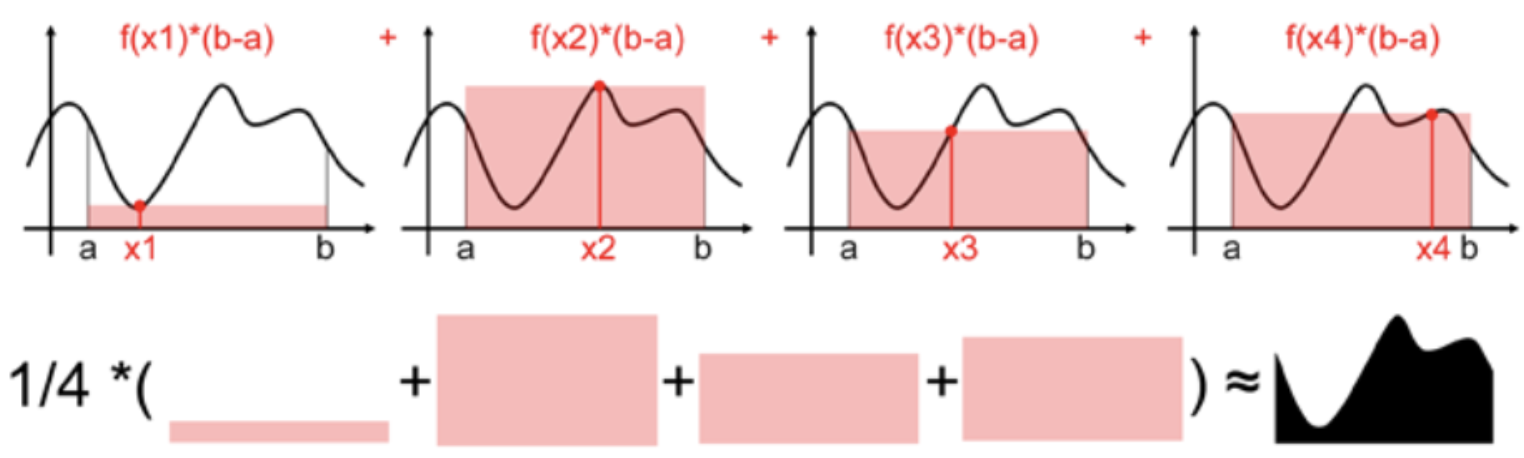
\includegraphics[width=0.9\linewidth]{Figure/Week 10/Monte Carlo visually.png}
    \caption{Monte Carlo visually}
\end{figure}

\subsection{Monte Carlo Methods}

\indent

\subsubsection{Monte Carlo estimation of $\pi$}

\indent 

Randomly draw $N$ points within unit square at random. Count the $R$ points which are inside the unit circle. Compute the ratio $R/N$ and estimate $\pi$ as $4R/N$.

In this example, the mathematical statistics of the procedure is:

Write the parameter we want to estimate, i.e., $pr$, as an expectation. Represent the parameter as a sample approximation. Let $f(\cdot)$ be the probability density function (pdf) of $X$ and $A$ be the support of $X$.

\begin{align*}
    \mathbb{E}[X] = \int _A tf(t)dt\approx \frac{1}{N}\sum_{i=1}^N X_i
\end{align*}

The law of large numbers guarantees that as the number of samples we draw increase, the estimator converges to the true parameter value almost surely.

We can replace $X$ with a function $g(X)$. Then the previous equation becomes:

\begin{align*}
    \mathbb{E}[g(X)] = \int_A g(t)\cdot f(t)dt\approx \frac{1}{N}\sum_{i=1}^N g(X_i)
\end{align*}

Here, we assume to draw $X_i \sim f$.

\subsubsection{Monte Carlo Integration example}

\indent 

One example is: $g(x) = e^{-x^2/2}$. $X_i$ is a uniform random variable on $(0,1)$. Then:

\begin{align*}
    \mathbb{E}[g(X)] = \int_0^1 e^{-x^2/2}dx\approx \frac{1}{N}\sum_{i=1}^N g(X_i)
\end{align*}

Goal is to evaluate the following definite integral: $\int_0^1 e^{-x^2/2}dx\approx \frac{1}{N}\sum_{i=1}^N g(X_i)$. Find a random variable such that the above holds. Need to be careful such that: Domain of the random variable and $g$ agree with the above definition.

\subsubsection{Simulating random variable}

\indent 

Let’s say we know how to simulate random variables that has a uniform distribution on the interval $[0,1]$. Call this uniformly distributed random variable $U$. Can do that in \texttt{R} with \texttt{runif}.

In \texttt{R}, we can draw random Gaussian variables using the function \texttt{rnorm}, but how do these functions really work? Two methods (others exist):

\begin{itemize}
    \item Inverse-transform method
    \item Acceptance-rejection method
\end{itemize}

Disadvantages of Simulating:

\begin{itemize}
    \item Inefficient when targeting rare events or small regions of the space.
    \item Scales poorly with dimensionality (curse of dimensionality)
    \item No adaptive as each sample is independent–no feedback or learning from previous samples.
\end{itemize}

\bigskip

\noindent \textbf{Inverse-transform method}:

Let’s say $X$ is a random variable that has a cumulative distribution function (cdf) $F$. Remember that cdf is the integral of the pdf:

\begin{align*}
    F(x) = \int_{-\infty}^x f(t)dt
\end{align*}

Recall $U$ is a uniformly distributed random variable over $[0,1]$. If the inverse of $F(x)$ exists, then we can generate $X$ as: $X=F^{-1}(U)$.

The exponential distribution has a pdf of the form:

\begin{align*}
f(x) = 
    \begin{cases}
        \lambda e^{-\lambda x} & \text{if } x>0\\
        0 & \text{if }x\leq 0
    \end{cases}
\end{align*}
    
and a cdf of the form:

\begin{align*}
F(x) = 
    \begin{cases}
        1- e^{-\lambda x} & \text{if } x>0\\
        0 & \text{if }x\leq 0
    \end{cases}
\end{align*}

The inverse cdf is:

\begin{align*}
    F^{-1}(p) = -\frac{\log(1-p)}{\lambda}, 0<p<1
\end{align*}

To sample from the exponential distribution, we can do the following:

\begin{itemize}
    \item Sample $U\sim \text{Uniform}(0,1)$
    \item Set $X = -\frac{\log(1-U)}{\lambda}$
\end{itemize}

\bigskip

\noindent \textbf{Acceptance-Rejection method}:

The problem with the inverse transform method is that you need to know the functional from of the inverse of the cdf. Acceptance-rejection method is a more general method can simulate “difficult” distributions.

Given two probability densities $f(x)$ and $g(x)$, with $f(x)<Mg(x)$ for all $x$. If $g(x)$ is a distribution that can be easily sampled, then we can sample $f(x)$ using the following procedure:

\step Draw a random variable $X\sim g(x)$.

\step Accept $X$ with probability $\frac{f(x)}{Mg(x)}$

\step Repeat steps 1 and 2 until you have the desired number of random samples

Problems with the Acceptance-rejection method: The envelop distribution $g(x)$ needs to closely resemble $f(x)$ for this method to work well.

If $g(x)$ does not match $f(x)$ well: The method will draw a lot of unwanted samples hence is not very efficient. Become very problematic when the data are high-dimensional. Even at dimensions of $\sim 10$, this method becomes very inefficient, i.e., you need to draw lots of samples before one sample is accepted.

\subsection{Monte Carlo simulation examples}

\subsubsection{Pop Mart Blind Box}

\indent 

Each Pop Mart Monster blind box costs \$22. There are 10 unique figures in the full set. Each box contains one random figure. How many boxes would you need to purchase — and how much money would you expect to spend — to collect all 10 figures?

\bigskip

\noindent\textbf{Analytical Solution (before we see the Monte Carlo)}:

Expected number of shops you need to do:

\begin{align*}
    \mathbb{E}[T] = n(\frac{1}{1}+\frac{1}{2}+\ldots + \frac{1}{n}) \approx n\log n+0.5772n+0.5
\end{align*}

where $T$ is the number of shops you need to do, and $n$ is the number of items to collect.

For the example, we have $n=10$ (the number of unique figures) so $E[T]≈30$. On average, you need to buy about 30 boxes.

\bigskip

\noindent\textbf{Monte Carlo Simulation}:

Using in \texttt{R}, the results is 29.733.

\subsubsection{Polya urn problem}

\indent

Let an urn start with 1 black ball and 1 white ball. Repeatedly draw a single ball from the urn. Each time a ball is drawn: You put back that ball plus one extra ball of the same colour back into the urn.

After 1000 draws, how many black balls do you expect to be in the urn? This is an example of using Monte Carlo to simulate a process.

\subsubsection{Call Option Pricing}

\indent

An European call option gives you the right to buy a stock at a particular price at expiry. 

Example: 90 day call option of a stock with \$105 strike. Let’s say a stock is currently priced at \$100. If it hits \$108 at day 90, then you can exercise the option and make a \$3 profit from this stock. If its price is below \$105 at day 90, then you make nothing.

Question: How much should you pay for this option today? Think of this as the insurance premium you’d pay to guarantee the right to buy later at a known price. A put option gives you the right to sell a stock at a particular price at expiry.

At expiration, the payoff of the call option is: $\text{Payoff} = \max (S_T - K,0)$, where $S_T$ is the stock price at expiry and $K$ is the strike price.

\noindent\textbf{Simulate stock price as a random (stochastic) model}:

Equation for the future price $S$ of a stock: $dS = S(\mu dT+\sigma\sqrt{dT}\mathcal{N})$, where $\mu$ is the growth rate of the stock price, $\sigma$ is known as the volatility (Think of this as the variance of the stock price), $\mathcal{N}$ is a standard normal random variable, $dT$ is one unit of time.

\noindent\textbf{Monte Carlo Simulation}:

\step Simulate many possible future stock prices $S_T$  based on the above equation.

\step For each simulation, calculate payoff.

\step The price you are willing to pay is the expected value of the payoff $E(\text{Payoff})$.


\pagebreak

\section{Week 11 - Markov Chain Monte Carlo}
\indent

Markov Chain Monte Carlo (MCMC) is a Monte Carlo sampling technique for generating samples from an arbitrary distribution.

The samples are not independent, but from a Markov chain where the future depends on upon the present.

Two popular implementations of MCMC are:

\begin{itemize}
    \item Metropolis-Hastings algorithm and generalization by Hastings
    \item Gibbs samplers
\end{itemize}

\subsection{Markov Chain}

\indent 

Markov chain is a random (stochastic) process that follows the Markov property. Markov property means that the future state of the process only depends on the current state. Consider a sequence $\{X_1,\ldots,X_n\}$, probabilities $P(X_n|X_{n-1},\ldots,X_1) = P(X_n|X_{n-1})$.

Three key components:
\begin{itemize}
    \item \textbf{State space}: Set of all possible states
    \item \textbf{Transition matrix}: Probabilities of moving from one state to another
    \item \textbf{Random sequence}: A sequence of random variables $(X_0,X_1,\ldots,)$
\end{itemize}

\subsubsection{Modelling Future Weather Conditions}

\indent 

\begin{figure}[h!]
    \centering
    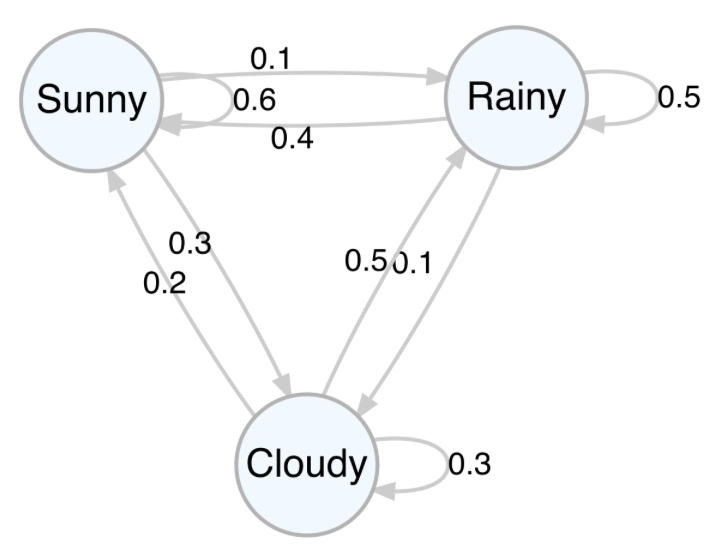
\includegraphics[width=0.5\linewidth]{Figure/Week 11/Modelling Future Weather Conditions.png}
    \caption{Modelling Future Weather Conditions}
\end{figure}

The state space is $S=\{\text{Sunny,Cloudy,Rainy}\}$, represented as the vertices of the graph. Edges represent the probability of moving from one state to another state. Example: if it is sunny today, 10\% chance of being rainy tomorrow.

The transition matrix $P$ is a $3\times 3$ matrix. Rows represent current state
Columns represent next state. $P_{ij}$ : probability of transiting from state $i$ to state $j$. Row of $P$ $\sum P_{i} = 1$.

\begin{align*}
    P = 
    \begin{pmatrix}
        0.6 & 0.1 & 0.3\\
        0.4 & 0.5 & 0.1\\
        0.2 & 0.5 & 0.3
    \end{pmatrix}
\end{align*}

This sequence is called a Markov Chain because each day’s weather only depends on today’s weather, not the entire history.

\subsubsection{Invariant (Stationary) Distribution}

\indent 

An invariant distribution is a probability distribution $\pi$ such that: $\pi = \pi P$ and $\pi \mathbf{1} = 1$.

If the system starts in distribution $\pi$, it stays in distribution $\pi$ after any number of transitions. It represents the long-term behavior of the Markov Chain. This is satisfied if the Markov chain is: Irreducible or Aperiodic.

\subsubsection{Irreducible}

\indent 

A Markov chain or transition matrix $P$ is said to be irreducible if there is some way of getting from state $i$ to state $j$, AND there is some way of getting from state $j$ to state $i$, $\forall i,j\in S$.

Consider the following transition matrix:

\begin{align*}
    P = 
    \begin{pmatrix}
        0 & 1 & 0\\
        0 & 0 & 1\\
        1 & 0 & 0
    \end{pmatrix}
\end{align*}

The chain cycles through: $1\rightarrow 2\rightarrow 3\rightarrow1\rightarrow 2\rightarrow 3\rightarrow\ldots$. You can return to the starting state only after $3, 6, 9, \ldots$ steps. Thus, \textbf{greatest common divisor} $\textbf{(gcd)}(3,6,9,...)=3$. All states are periodic with period 3.

\subsubsection{Aperiodic}

\indent 

Suppose we modify the transition matrix:

\begin{align*}
    P = 
    \begin{pmatrix}
        0.1 & 0.9 & 0\\
        0 & 0.5 & 0.5\\
        0.4 & 0 & 0.6
    \end{pmatrix}
\end{align*}

The state is aperiodic, meaning returns can happen more irregularly without being locked into a repeating cycle. Now can return in $1, 2, 3, 4, \ldots$ steps. $\textbf{gcd}(1,2,3,4,\ldots)=1$.

\subsubsection{The Use of Invariant Markov Chain}

\indent 

Similar to Monte Carlo, our main interest here continues to be the simulation of $X_1,X_2,\ldots$, that follow (or approximately follow) the distribution with density $f(x)$ where directly simulating from $f(x)$ is difficult.

This problem is ubiquitous in Bayesian statistics.

\begin{itemize}
    \item Frequentist statistics: there exist true parameters ($\boldsymbol{\theta}$ is fixed but unknown).
    \item Bayesian statistics: all model parameters are random variables.
\end{itemize}

For Bayesian statistics, the model parameters $\boldsymbol{\theta}$ has a prior distribution.

Given data $\mathbb{D}$, we want to compute the posterior distribution $p(\boldsymbol{\theta}|\mathbb{D})$.

\begin{align*}
    p(\boldsymbol{\theta}|\mathbb{D}) = \frac{p(\mathbb{D}|\boldsymbol{\theta})p(\boldsymbol{\theta})}{\int p(\mathbb{D}|\boldsymbol{\theta'})p(\boldsymbol{\theta'})d\boldsymbol{\theta'}}
\end{align*}

Generally, it’s very difficult to exactly compute $p(\boldsymbol{\theta}|\mathbb{D})$. Sample from $p(\boldsymbol{\theta}|\mathbb{D})$: using MCMC

Idea: construct a Markov chain such that its stationary distribution is the desired posterior distribution $p(\boldsymbol{\theta}|\mathbb{D})$.

\subsection{MCMC - Metropolis-Hasting algorithm}

\indent 

Imagine you are a politician trying to visit all the town halls in your electorate. Imagine there are four town halls: A, B, C, and D. Each town hall has a different number of voters. Your goal: Spend time at each town hall proportional to its voter population.

\begin{table}[h!]
    \centering
    \begin{tabular}{ccc}
        \hline
        \textbf{Town Hall} & \textbf{Number of Voters} & \textbf{Proportion (Target $f(x)$}\\\hline
        A & 500 & 0.25\\
        B & 1000 & 0.5\\
        C & 300 & 0.15\\
        D & 200 & 0.10\\\hline
    \end{tabular}
\end{table}

\step Start at a random town hall.

\step Propose moving to a randomly chosen new town hall.

\step Accept or reject the move:
\begin{itemize}
    \item If the new hall has more voters $\rightarrow$ Always accept.
    \item If fewer voters $\rightarrow$ Accept with probability
\end{itemize}

\begin{align*}
    \text{Accept probability} = \min \left(1,\frac{\text{Number of people in new town hall}}{\text{Number of people in current town hall}}\right)
\end{align*}

\step Repeat the process for a large number of steps (e.g., 10000).

\step Track the proportion of time spent in each town hall.

\subsubsection{Explanation}

\indent 

Similar to the acceptance-rejection method. It simulates a trial state. Accepts or rejects the trial state according to some random mechanism

Uses the Markov chain because each trial state depends on the previous state – Almost memory-less system. Aim is to construct a Markov chain $\{X_t,t=0,1,\ldots\}$ such that the limiting distribution is $f(x)$.

\subsubsection{Generalisation}

\indent 

We want to simulate samples from a complicated target distribution $f(x)$, which might be difficult to sample from directly.

\noindent \textbf{Basic Steps}:

\step Start with an initial state $X_0$.

\step Propose a new point $Y$ based on the current point $X_t$, using a proposal distribution $q(y|x)$.

\step Accept or reject the proposal $Y$ according to an acceptance probability $\alpha(X_t,Y)$.

This way, even if $q$ isn’t perfect, we still eventually generate samples that have the correct distribution $f(x)$ when it reaches stationarity.

\begin{algorithm}[H]
\caption{Metropolis-Hastings algorithm}
\begin{algorithmic}
    \For{$t=0,1,\ldots, N-1$}
        \State Draw $Y\sim q(x|X_t)$.
        \State Calculate acceptance probability $\alpha(X_t,Y)$.
        \State Define $\alpha(x,y) = \min\{\frac{f(y)q(x|y)}{f(x)q(y|x)},1\}$.
        \State Draw $U\sim \text{Uniform} (0,1)$.
        \State If $U\leq \alpha$ then $X_{t+1} \leftarrow Y$ else $X_{t+1}\leftarrow X_t$
    \EndFor
    \Ensure $X_1,X_2,\ldots,X_N$
\end{algorithmic}
\end{algorithm}

\subsubsection{Symmetric Proposal Function}

\indent 

If the proposal density function is $\textbf{symmetric}\Rightarrow q(y|x) = q(x|y)$. The acceptance probability has a simpler form. The MCMC algorithm is also known as a random walk sampler.

One common choice of a symmetric proposal function is just the Gaussian function, i.e., $q(x)\sim \mathcal{N}(x_t,\sigma)$. The choice of $\sigma$ affects how quickly the state space is explored.

\subsection{Applications of MCMC}

\indent

One common application of MCMC is to draw from the posterior distribution in Bayesian statistical methods.

\begin{align*}
    \textcolor{red}{P(A|B)} = \textcolor{blue}{\frac{P(B|A)}{P(B)}}\textcolor{orange}{P(A)}
\end{align*}

\begin{itemize}
    \item Posterior $\textcolor{red}{P(A|B)}$: The likelihood of $A$ occurring given $B$ has occurred.
    \item Likelihood ratio $\textcolor{blue}{\frac{P(B|A)}{P(B)}}$: The support $B$ provides for $A$.
    \item Prior $\textcolor{orange}{P(A)}$: The probability of $A$ before any data are gathered.
\end{itemize}

\subsubsection{The posterior distribution}

\indent 

Can use the Bayes rule for modelling and data.

\begin{align*}
    \textcolor{red}{P(\boldsymbol{\theta}|\mathbb{D})} = \textcolor{blue}{\frac{P(\mathbb{D}|\boldsymbol{\theta})}{P(\mathbb{D})}}\textcolor{orange}{P(\boldsymbol{\theta})}
\end{align*}

\begin{itemize}
    \item Posterior $\textcolor{red}{P(\boldsymbol{\theta}|\mathbb{D})}$: The likelihood of $\boldsymbol{\theta}$ occurring given the data $\mathbb{D}$.
    \item Likelihood ratio $\textcolor{blue}{\frac{P(\mathbb{D}|\boldsymbol{\theta})}{P(\mathbb{D})}}$: The support $\mathbb{D}$ provides for $\boldsymbol{\theta}$.
    \item Prior $\textcolor{orange}{P(\boldsymbol{\theta})}$: The probability of $\boldsymbol{\theta}$ before any data are gathered.
\end{itemize}

Typically $p(\mathbb{D})$ is a difficult integral to evaluate:

\[
p(\mathbb{D}) = \int P(\mathbb{D}|\boldsymbol{\theta}) p(\boldsymbol{\theta})d\boldsymbol{\theta}
\]

\subsubsection{MCMC for Estimating Regression Models}

\indent 

\begin{align*}
    \textcolor{red}{P(\boldsymbol{\theta}|\mathbb{D})} = \textcolor{blue}{\frac{P(\mathbb{D}|\boldsymbol{\theta})}{P(\mathbb{D})}}\textcolor{orange}{P(\boldsymbol{\theta})}
\end{align*}

\begin{align*}
    & Y = \beta_0+\beta_1X_1+\ldots+\beta_pX_p+\epsilon; & \epsilon\sim \mathcal{N}(0,\sigma^2)
\end{align*}

\begin{itemize}
    \item $\boldsymbol{\theta} = \{\beta_0,\beta_1,\ldots,\beta_p,\sigma^2\}$
    \item $\mathbb{D} = \{Y_1,Y_2,\ldots,Y_n,X_{11},X_{12},\ldots,X_{np}\}$
    \item $p(\mathbb{D}|\boldsymbol{\theta})$ will be Gaussian
    \item $p(\mathbb{D})$ is not so easy to compute
    \item $p(\boldsymbol{\theta})$ is the chosen prior
\end{itemize}

Recall the acceptance probability in the Metroplos-Hasting algorithm is:

\[
\alpha(x,y) = \min\left\{\frac{f(y)q(x|y)}{f(x)q(y|x)},1\right\}
\]

Assume the proposal density is symmetric, i.e.,  $q(y|x) = q(x|y)$. My target density $f$ is now the posterior distribution, i.e., $p(\boldsymbol{\theta}|\mathbb{D})$. Then in the Metropolis-Hastings algorithm, we only need to calculate:

\[
\alpha = \frac{p(\boldsymbol{\theta'|\mathbb{D}})}{p(\boldsymbol{\theta}|\mathbb{D})}=\frac{p(\mathbb{D}|\boldsymbol{\theta')}p(\boldsymbol{\theta'})}{p(\mathbb{D}|\boldsymbol{\theta})p(\boldsymbol{\theta})}
\]

Since $p(\mathbb{D)}$ doesn’t depend on $\boldsymbol{\theta}$, it cancels out on the right hand side of the above formula and hence it isn’t included in the formula.

\subsubsection{MCMC for Estimating $P(\text{Head})$ of a coin flip}

\indent 

Observe a series of coin flips: H, T, H, H, T, H, T, H, H, T, H, H, H, T, H, H, H, T, H, H, $\ldots$. $\theta = P(\text{Head})$

Frequentist perspective: $\theta$ is fixed but unknown.

Bayesian perspective: $\theta$ is a random variable; one can compute the likelihood of $\theta$ given the observed data.

$\theta_0$ set as an initial point. Compute $\theta_t$ as a Markov chain. Use MCMC algorithm to estimate the posterior distribution of $\theta$.

\subsubsection{MCMC practical considerations}

\indent 

The samples at the start of the MCMC, before the algorithm converges to the true distribution are known as the burn-in period. It should be discarded.

The samples generated by MCMC are correlated since they are from a Markov chain
Previously, many practitioners advocated thinning the samples by taking say every $k^{th}$ sample. 

This was done for a few reasons historically. Reduce correlations and compute standard errors more easily. Less space needed to store the chain.

\pagebreak


\end{document}
